\documentclass[doktyp=barbeit, sprache=german]{TUBAFarbeiten}
\usepackage[utf8]{inputenc}
\usepackage[T1]{fontenc}
\usepackage{graphicx} 
\usepackage{amsmath}
\usepackage{subcaption}
\usepackage[Algorithmus]{algorithm}
\usepackage{algorithmicx}
\usepackage[noend]{algpseudocode}
\usepackage[numbers]{natbib}
\usepackage{booktabs}
\usepackage{rotating}
\usepackage{lscape}
\usepackage{mwe}
\usepackage{listings}
\usepackage{xcolor}
\usepackage{amssymb}
\usepackage{url}

\newcommand*\rfrac[2]{{}^{#1}\!/_{#2}}

\lstset { %
    language=C++,
    backgroundcolor=\color{black!5}, % set backgroundcolor
    basicstyle=\footnotesize,% basic font setting
    numbers=left
}



\captionsetup{justification=centering}
\captionsetup{compatibility=false}
\bibliographystyle{unsrt}
\TUBAFFakultaet{Fakultät für Mathematik und Informatik}
\TUBAFInstitut{Institut für Informatik}
\TUBAFLehrstuhl{Lehrstuhl für Künstliche Intelligenz und Datenbanken}
\TUBAFTitel{Eine Studie zur kombinatorischen Optimierung mit Ameisenalgorithmen}
\TUBAFBetreuer{Prof. Dr. H. Jasper}
\TUBAFKorrektor{M. Sc. V. Göhler}
\TUBAFAutor[S. Dressel]{Samuel Dressel}
\TUBAFStudiengang{Angewandte Informatik}
\TUBAFVertiefung{Künstliche Intelligenz}
\TUBAFMatrikel{59963}
\TUBAFDatum{\today}
\begin{document}
\maketitle
\TUBAFErklaerungsseite
\section*{Danksagung}
\thispagestyle{empty}
An dieser Stelle möchte ich mich bei all denjenigen bedanken, die mich während der Anfertigung dieser Bachelorarbeit unterstützt und begleitet haben. Zuerst gebührt mein Dank dem 2. Korrektor Volker Göhler, der viel Zeit in eine hilfreiche Betreuung investiert hat und mir mit konstruktiven Anregungen zur Seite stand. Desweiteren möchte ich meinem Betreuer, Prof. H. Jasper, für die unkomplizierte Hilfe bei der Organisation meiner Arbeit danken. Der Dank für eine schnelle Korrekturlesung dieser Arbeit gilt Constanze Bragulla.
\\Abschließend danke ich meiner Familie, die mich während des Studiums sehr unterstützt hat und Gott, dessen Segen ich in den vergangenen Jahren immer wieder spüren durfte.
\\\\\\Samuel Dressel
\\Freiberg den \today
\newpage
\tableofcontents
\newpage
\section{Einleitung}
Die kombinatorische Optimierung als Teilgebiet der diskreten Mathematik und die darin enthaltenen Probleme haben in den vergangenen Jahrzehnten mehr und mehr an Bedeutung in Industrie, Wirtschaft und Forschung gewonnen. Wie der Name \glqq Kombinatorische Optimierung\grqq\, schon sagt, geht es darum, in unterschiedlichen Anwendungen Kosten in vielerlei Ausprägung zu minimieren und zu optimieren. Der Begriff \glqq Kosten\grqq\r steht dabei stellvertretend für Optimierungsgrößen wie Weglängen, Gewichtungen oder auch finanzielle Mittel.
\\Ein prominentes Szenario der kombinatorischen Optimierung ist das Travelling Salesman Problem, zu Deutsch: \glqq Problem des Handlungsreisenden\grqq\,. Hierbei der Besuch mehrerer Städte so gewählt werden, dass keine Stadt mehrmals besucht wird, die gesamte Reisestrecke möglichst kurz ist und die Reise letztendlich wieder in der Anfangsstadt endet. Eine naheliegende Anwendung ist hierbei die Tourenplanung in der Logistik, jedoch findet sich das Problem auch bei der Herstellung von Mikrochips \cite{Microchip} oder auch bei der Genom-Sequenzierung \cite{DNA} wieder. Die Begriffe \glqq Stadt\grqq\, und \glqq Routenlänge\grqq\, sind in diesen Fällen dann nur repräsentativ. Im Fall der Genom-Sequenzierung stellen die Städte die DNA-Teilstränge dar, bei der Herstellung von Mikrochips die Bohrlöcher.
\\Aufgrund der Wichtigkeit dieses Problems haben sich in der Vergangenheit viele Wissenschaftler damit beschäftigt, effektive Algorithmen für die Lösung des TSP zu entwerfen. Mittlerweile gibt es deswegen eine Reihe von schnellen und effizienten Algorithmen. Zum einen sind das exakte Verfahren, deren Umsetzung den Namen \glqq Direktlöser\grqq\, trägt. Hierbei ist zum Beispiel der \textit{Concorde TSP Solver} \cite{ConcordeMain} zu erwähnen, der auch größere Probleme in einer aktzeptablen Zeit löst und das optimale Ergebnis findet. Ein andere Möglichkeit, eine TSP-Instanz zu lösen, sind heuristische Algorithmen. Diese finden bei größeren Probleme zwar meist nur eine näherungsweise optimale Lösung, benötigen dafür aber nur sehr wenig Zeit. Eine solche Möglichkeit, das TSP heuristisch zu lösen, ist der Ameisenalgorithmus.
\\In dieser Arbeit soll die Anwendung dieses Ameisenalgorithmus auf die Lösung des TSP erklärt und für verschiedene Implementierungen in der objektorientierten Programmiersprache C\texttt{++} untersucht werden. Dabei werden im folgenden Kapitel \ref{sec:Grundlagen} die mathematischen und biologischen Grundlagen erklärt. Danach wird auf die Implementierung eingegangen und die Funktionsweise der Algorithmen diskutiert (Kapitel \ref{sec:Implementierung}). Anschließend wird in den Kapiteln 4 und 5 der Durchlauf der Experimente zu diesen Implementierungen vorgestellt und ausgewertet. Kapitel 6 gibt dann eine Zusammenfassung und einen Ausblick über die Verwendung des Ameisenalgorithmus zur Lösung des Travelling Salesman Problem und stellt Vor- und Nachteile sowie Möglichkeiten für zukünftige Forschungsprojekte vor.
\newpage
\section{Grundlagen}
\label{sec:Grundlagen}
In diesem Kapitel werden die benötigten theoretischen Grundlagen definiert. Dabei wird zunächst auf den Ameisenalgorithmus und das Travelling-Salesman-Problem (TSP) im Einzelnen eingegangen. Abschließend wird die Herangehensweise zur Lösung des TSP mit dem Ameisenalgorithmus erklärt.
\subsection{Der Ameisenalgorithmus (Ant Colony Optimization)}
\subsubsection{Biologische Grundlagen}
Für das weitere Verständnis des \textit{Ameisenalgorithmus} (auch Ant Colony Optimization Algorithm oder kurz ACO) ist zunächst ein Blick auf die biologischen Grundlagen notwendig. Ein Tierstaat, wie er bei Ameisen zu finden ist, funktioniert nur mit einer effektiven und sinnvollen Kommunikation. Methoden zur Verständigung wie das Kommunizieren über Vibrationen und Berührungen sind eher die Ausnahme und kommen nur in speziellen Situationen zum Tragen \cite{Ameisen}. Dagegen kommt zum größten Teil der Informationsaustausch über Duftstoffe (sog. Pheromone) zur Anwendung. Diese werden durch verschiedene Drüsen erzeugt und wiederum in unterschiedlicher Kombination und Konzentration abgegeben.
Diese Pheromone werden benutzt, um Nestgenossen zu erkennen oder um bei Gefahren Kampf- und Abwehrverhalten auszulösen.
\\Hauptsächlich jedoch nutzen Ameisen die Pheromone, um eine Duftspur über ihren Hinterleib abzugeben. Diese dient dem Tierstaat als Orientierungshilfe. Zum einen werden damit Straßen zu anderen Kolonien gebildet, zum anderen dienen sie dazu, anderen Ameisen den Weg zu einer Nahrungsquelle zu zeigen. Die Tatsache, dass ein Weg mit einer höheren Pheromonkonzentration bevorzugt wird, ist Grundlage des Ameisenalgorithmus.
\subsubsection{Der Ameisenalgorithmus}
Der historische Ursprung des Algorithmus findet sich in den Versuchen von Jean-Louis Deneubourg und seinen Kollegen \cite{Biological}. Das sogenannte \glqq Double-Bridge-Experiment\grqq \,zeigte, dass Ameisen den kürzesten Weg aufgrund der Pheromonmarkierung finden. 
\\In diesem Experiment ist eine Kolonie von Argentinischen Ameisen mit einer Nahrungsquelle durch zwei Brücken verbunden, die gleichzeitig die einzigen Zugänge zu dieser Nahrungsquelle bilden \cite{Dorigo2007}. Im ersten Teil des Versuchs sind diese beiden Brücken jeweils gleich lang (siehe Abbildung \ref{img:DBExperiment}a). Zu Beginn erkunden die Ameisen die Umgebung der Kolonie, bis sie eine Entscheidung über die Auswahl der Brücke treffen müssen. Lässt sich aufgrund einer noch nicht stattgefundenen Begehung der Brücken keine Pheromonspur feststellen, so entscheiden die Ameisen rein zufällig, welche Brücke sie wählen. Die Wahrscheinlichkeit für beide Wege liegt bei gleichen Bedingungen bei je 50 Prozent. Wird der Versuch über längere Zeit durchgeführt, so wird durch Zufall die Pheromonkonzentration der einen Brücke höher sein als die der anderen. Diese wird dadurch attraktiver für die Ameisen und wird somit letzten Endes der favorisierte Weg zur Nahrungsquelle. 
\\Im zweiten durchgeführten Versuch sind die beiden Brücken unterschiedlich lang (siehe Abbildung \ref{img:DBExperiment}b). Auch hier liegt die Wahrscheinlichkeit für beide Brücken zu Anfang bei je 50 Prozent. Da die Ameisen, die sich für die kürzere Brücke entscheiden, schneller wieder zurück am Nest sind, steigt das Pheromonlevel auf diesem Weg deutlich schneller an. Nach einiger Zeit kristallisiert sich die kürzere Brücke als optimale Route heraus, während der längere Weg durch eine natürliche Pheromonverdunstung immer unattraktiver wird. Im Vergleich zum ersten Versuch geschieht der Ausbau der Pheromonspur wesentlich schneller und effektiver.
\begin{figure}
\captionsetup[subfigure]{justification=centering}
\centering
\begin{subfigure}[c]{0.45\textwidth}

\includegraphics[width=0.9\textwidth]{images/RouteTrivial.png}
\subcaption{Skizze zu Versuch 1; beide Wege sind gleich lang}
\end{subfigure}
\begin{subfigure}[c]{0.45\textwidth}
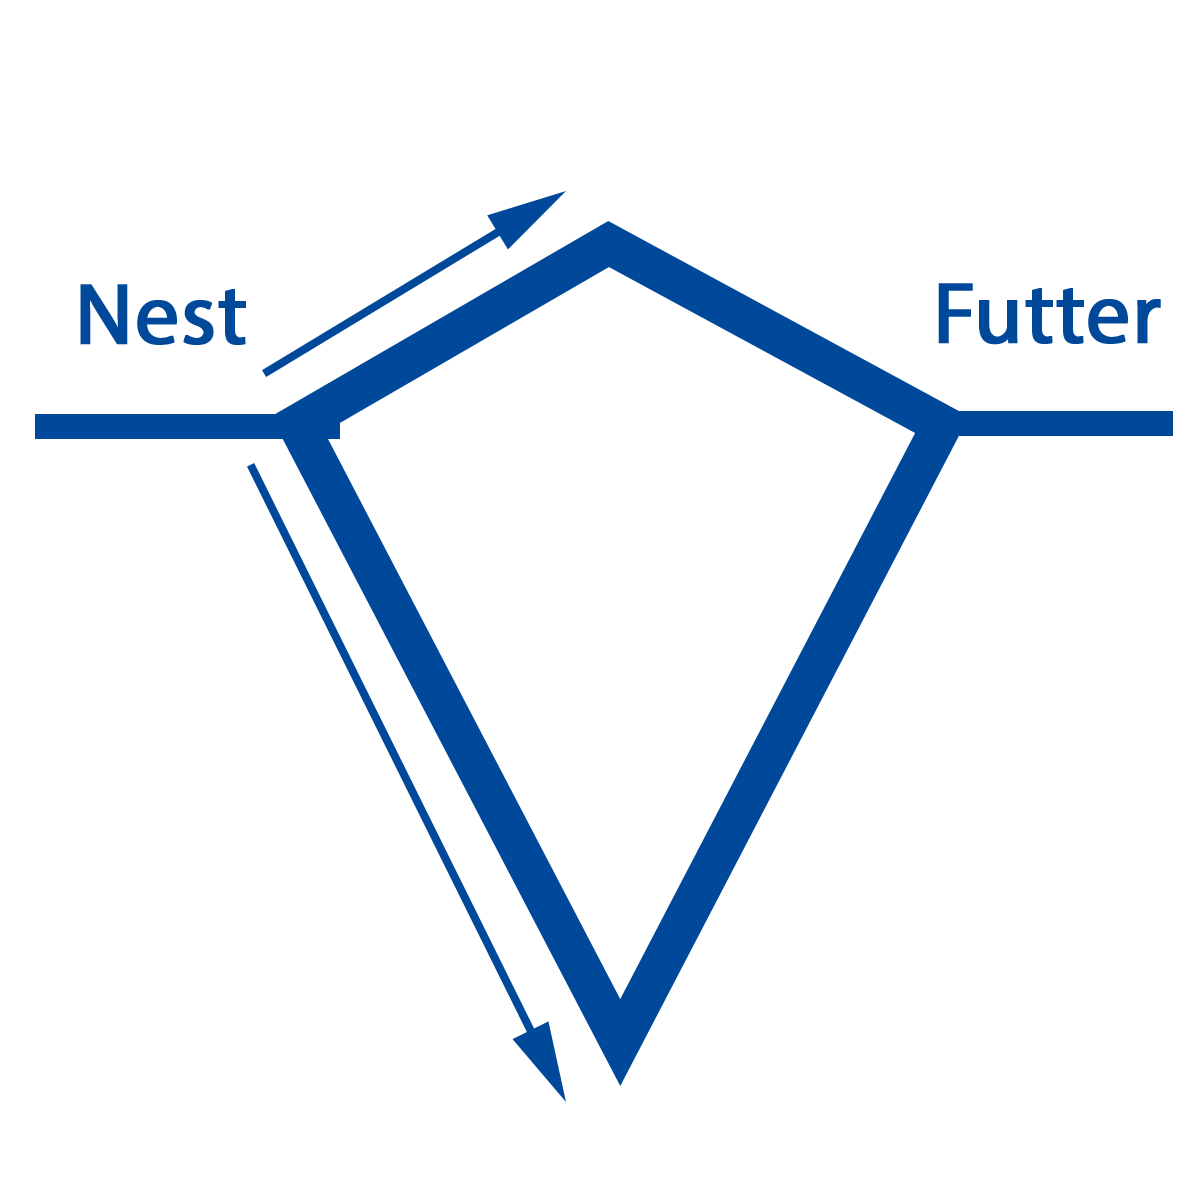
\includegraphics[width=0.9\textwidth]{images/RouteAdv.png}
\subcaption{Skizze zu Versuch 2; die Wege sind unterschiedlich lang}
\end{subfigure}
\caption[Double-Bridge-Experiment nach Deneubourg]{Double-Bridge-Experiment nach Deneubourg \cite{Biological}}
\label{img:DBExperiment}
\end{figure}
\subsection{Das Travelling-Salesman-Problem}
\subsubsection{Das Problem im Allgemeinen}
Das \textit{Travelling Salesman Problem} (im Folgenden mit TSP abgekürzt) ist eines der bekanntesten und am meisten  untersuchten Optimierungsprobleme \cite{TaschenbuchAlgorithmen}. Kerninhalt des Problems ist dabei folgender: Ein Handlungsreisender soll in einer Rundreise \(n\) verschiedene Städte besuchen. Der Reisende startet dabei (zufällig) in einer dieser Städte und am Ende seiner Reise kehrt er auch wieder in diese Stadt zurück. Dabei sollen alle $n$ Städte nur einmal besucht werden und die Weglängen bzw. die Kosten der gesamten Reise minimal sein.
\\Seinen geschichtlichen Ursprung hat das TSP im Jahr 1832, als in Deutschland ein Buch mit dem Titel \glqq Der Handlungsreisende, wie er sein soll und was er zu thun hat, um Aufträge zu erhalten und eines glücklichen Erfolges in seinen Geschäften gewiss zu sein\grqq\, erschien. Dieses Buch und dessen Inhalt diente als Grundlage für die Erforschung des Problems. Die erste Benutzung des Ausdrucks \glqq Travelling Salesman Problem\grqq\, erfolgte in mathematischen Kreisen etwa um das Jahr 1931 \cite{TSP}. 
Dies geschah, als mehrere amerikanische Mathematiker sich des Problems annahmen \textendash{} wichtige Vertreter waren dabei Merrill Flood und Hassler Whitney, die die Überlegungen des österreichischen Mathematikers Karl Menger als Grundlage nahmen. Nach und nach wurde das Problem durch zahlreiche Veröffentlichungen immer präsenter und bis heute ist dies bis heute noch.
\subsubsection{Graphentheoretische Grundlagen} \label{graphbasics}
Um das Problem formal als ein graphentheoretisches Problem darzustellen, werden im Folgenden die dafür benötigten Begriffe definiert. Diese Definitionen finden sich unter anderem in \cite{graphKemnitz} und \cite{graphDiestel}.
\\\\$G = (V,E,c)$ sei zunächst ein \textit{ungerichteter Graph}. Dabei beschreibt $V = \{1,...,n\}$ die Menge der Knoten und $E$ die Menge der Kanten, welche letzten Endes eine Menge von ungeordneten Paaren $e \in E = \{i,j\}$ mit $i,j \in V$ ist. $c$ beschreibt die Gewichtung der einzelnen Kanten in $E$. Das Attribut \textit{ungerichtet} beschreibt die Eigenschaft des Graphen $G$, dass die Menge $E$ eine ungeordnete Menge ist.
\\\\Ist $e = ij = \{i,j\}$ eine Kante von $G$, dann verbindet $e$ die Knoten $i$ und $j$. Diese Knoten $i,j$ heißen dann \textit{adjazent}. Die Kante $e$ dagegen heißt dann \textit{inzident} zu $i$ und $j$. 
\\\\Die Menge $N(v)$ aller Knoten von $G$, die zu $v$ adjazent sind, nennt man \textit{Nachbarschaft} von $v$.
\\\\Ein weiterer wichtiger Begriff ist der \textit{Grad} $d$ eines Knotens $v \in V$. Dabei ist der Grad $d(v)$ die Anzahl der zu $v$ inzidenten Kanten.
\\\\Eine \textit{Kantenfolge} $W = (v_0v_1,v_1v_2,...,v_{r-1}v_r)$ eines Graphen $G$ ist eine Folge von Kanten. Wenn alle Kanten in dieser Kantenfolge verschieden sind, dann heißt diese Folge \textit{Kantenzug}. Sind zudem noch alle Knoten paarweise verschieden, so erhält man einen \textit{Weg} $P$.
\\\\Gilt $v_0 = v_r$, so heißt der Weg geschlossen oder auch \textit{Kreis}.
\\\\Enhält so ein Kreis $C$ nicht unbedingt jede Kante $e$ von $G$, aber dafür jeden Knoten $v$ von $G$ genau einmal, so nennt man diesen Kreis einen \textit{Hamiltonkreis} $\pi$ (auch \textit{Tour}) von $G$. Ein Hamiltonkreis $\pi$ heißt dann \textit{optimal}, wenn die Summe der Kantengewichte minimal wird.
\\\\Existiert in $G$ ein Kantenzug $Z$, der alle Kanten enthält und zudem geschlossen ist, dann heißt $Z$ \textit{Eulertour} und $G$ \textit{eulerscher Graph}.
\\\\Für die Betrachtung von möglichen Lösungsalgorithmen des TSP müssen nun noch abschließend der Begriff des Baums und des Matchings definiert werden:
\\Ein \textit{Baum} ist ein zusammenhängender, kreisloser Graph. Ein Baum $T$ heißt \textit{Spannbaum} von $G$, wenn er $G$ ganz aufspannt, d. h. wenn $V(T) = V(G)$ ist. Der Spannbaum ist \textit{minimal}, wenn seine Länge minimal ist.
\\\\$M$ ist ein \textit{Matching} von $U \subseteq V$, wenn jeder Knoten $U$ mit einer Kante aus $M$ inzidiert.
\\\\Auf dieser mathematischen Grundlage lässt sich das TSP nun wie folgt definieren: 
\begin{quotation}
$G = (V,E,c)$ sei Graph und $F$ die Menge aller Hamiltonkreise in $G$. Ziel ist nun das Finden des Hamiltonkreises $f \in F$, für den die Summe der einzelnen Kantenkosten minimal wird \cite{TSPVariations}.
\end{quotation}
Unter der bislang unbewiesenen Annahme, dass die Komplexitätsklassen $P$ und $NP$ verschieden sind, gehört das TSP zur Klasse der NP-vollständigen Probleme, was bedeutet, dass es sich nicht mit einem deterministischen Algorithmus in Polynomialzeit lösen lässt \cite{Applegate2007}.  Alle ansatzweise effektiven Möglichkeiten und Algorithmen zur Lösung von TSP-Instanzen mit sehr vielen Städten basieren deshalb auf heuristischen Verfahren. Für Probleme mit wenigen Städten gibt es effektive Direktlöser, die das optimale Ergebnis in durchaus annehmbarer Zeit liefern.
\subsubsection{Ansätze und Algorithmen zur Lösung des Problems}
Da das Problem wie oben schon erwähnt zu den NP-vollständigen Problemen gehört, ist ein Algorithmus zur Lösung des TSP entweder schnell oder er findet eine optimale Tour - aber er wird nicht beide Eigenschaften besitzen \cite{TSP}. Deswegen unterscheidet man wie auch allgemein bei anderen kombinatorischen Optimierungsproblemen zwischen exakten und heuristischen Algorithmen.
Der einfachste Algorithmus zur exakten Lösung des TSP ist die sogenannte \textit{\glqq brute-force\grqq}- oder naive Methode \cite{TaschenbuchAlgorithmen}. Dieser Algorithmus betrachtet nacheinander alle möglichen Touren und deren Länge und ermittelt durch den Vergleich derselben die optimale und kürzeste Tour. 
\\Ist der Graph \(G\), der dieses Problem modelliert, ein ungerichteter Graph, so muss man mit diesem Algorithmus \(\frac{1}{2} \cdot (n - 1)!\) verschiedene Rundreisen betrachten. Bei neun verschiedenen Städten ergeben sich daraus 20160 verschiedene Touren, bei 16 Städten dagegen schon ca. 653 Milliarden Routen, dies macht den Algorithmus für die meisten Optimierungsprobleme völlig unbrauchbar. Auch andere exakte Methoden haben oft einen hohen Rechen- und Zeitaufwand. Man entscheidet sich deswegen häufig dafür, effiziente heuristische Algorithmen zu konstruieren, die zwar nicht immer eine optimale Tour finden, aber zumindest eine nahezu optimale Tour. Es existiert eine Vielzahl solch heuristischer Verfahren.
\\Eines der intuitivsten ist der \textit{Nearest-Neighbor-Algorithmus} \cite{Lotz2014}. Hierbei wird ein zufälliger Knoten $v_1$ als Startknoten ausgewählt. Danach wird iterativ immer der Knoten $v_i$ ausgewählt, der dem zuletzt ausgewählten Knoten $v_{i-1}$ am nächsten liegt und noch nicht in der schon besuchten Knotenmenge $V^\prime$ enthalten ist. Der Algorithmus ist beendet, wenn alle Knoten besucht wurden. Das Problem hierbei ist, dass die letzte Kante, die den letzten Knoten $v_{|v|}$ mit dem Startknoten $v_1$ verbindet und den Hamiltonkreis vervollständigt, eine mehr oder weniger beliebige Länge haben kann und somit das Erreichen einer möglichst kurzen Tourlänge wesentlich einschränken kann. Der Algorithmus ist formal in Algorithmus \ref{euclid} dargestellt.
\begin{algorithm}
\caption{Nearest Neighbor Algorithm}
\label{euclid}
\textbf{Eingabe:} $G = (V,E,c)$
\\\textbf{Ausgabe:} Tour $\pi$, die alle Knoten $v \in V$ besucht
\begin{algorithmic}[1]
\State $z_1 := v \in V$
\State $V^\prime := V \, \backslash \, \{v_1\}$
\State $i := 2$
\While {$V^\prime \ne \emptyset$}
\State $z_1 := min_{v\in V^\prime}  \, c(\{v_{i-1},v\})$
\State $V^\prime := V^\prime \, \backslash \, \{v_i\}$
\State $i := i +1 $
\EndWhile
\State $\pi := (v_1,...,v_n,v_1)$
\end{algorithmic}
\end{algorithm}
\\Ein weiterer bekannter heuristischer Algorithmus ist die \textit{Minimal-Spanning-Tree-Heuristik, kurz MST}. Dabei wird zunächst ein minimaler Spannbaum $T$ für den Graphen $G$ ermittelt \cite{Groetschel2005}. Zur Ermittlung dieses minimalen Spannbaumes stehen mehrere Algorithmen zur Verfügung (Algorithmus von Prim, Algorithmus von Kruskal, ...) \cite{MST}. Repräsentativ findet sich der Pseudocode für den Algorithmus von Prim in Algorithmus \ref{prim}. 
\\Die Konstruktion des minimalen Spannbaums erfolgt ausgehend von einem Startknoten $r$, welcher gleichzeitig der erste Knoten von $T$ ist. In jedem Schritt wird nun eine Kante mit minimalem Gewicht gesucht, die einen weiteren Knoten mit $T$ verbindet. Diese Kante $(u,v)$ wird zu $T$ hinzugefügt. Das Ganze wird solange wiederholt, bis alle Knoten $v \in V$ in $T$ vorhanden sind. 
\begin{algorithm}
\caption{Algorithmus von Prim}
\label{prim}
\textbf{Eingabe:} $G = (V,E,c)$
\\\textbf{Ausgabe:} Minimaler Spannbaum T
\begin{algorithmic}[1]
\State $T := \emptyset$
\State $r := v \in V$
\State $U := \{r\}$
\While {|U| < |V|}
\State Finde $u \in U$ und $v \in V - U$ mit $(u,v)$ ist minimal
\State $T := T + \{(u,v)\}$
\State $U := U + \{v\}$
\EndWhile
\end{algorithmic}
\end{algorithm}
\\Nach erfolgreicher Konstruktion des minimalen Spannbaums wird jede Kante innerhalb dieses Spannbaumes verdoppelt; es entsteht der eulersche Graph $G^\prime$. Nun wählt man einen beliebigen Startknoten und folgt den Kanten im Sinne einer Eulertour. Bereits besuchte Kanten werden dabei gestrichen und stattdessen die direkte Verbindung zwischen den jeweils verbleibenden Knoten gewählt. Das \textit{Verfahren von Christofides} baut auf diesem Algorithmus auf und erweitert diesen dadurch, dass der minimale Spannbaum nicht verdoppelt wird. Stattdessen wird das minimale Matching von den Knoten in $B$ gesucht, die einen ungeraden Grad haben. 
\\\\Nach der Dreiecksungleichung gilt, dass die Summe der Längen zweier Seiten $a$ und $b$ stets mindestens so groß ist wie die Länge der dritten Seite (formal: $c \leq a + b$). Die MST-Heuristik ist deswegen höchstens doppelt so lang, die Christofides-Heuristik höchstens 1,5-mal so lang wie die optimale Lösung \cite{Groetschel2005}.
\subsubsection{TSPLIB als Quelle für bekannte Probleme} \label{TSPLIB}
Die in dieser Arbeit untersuchten Probleminstanzen stammen aus der TSPLIB der Universität Heidelberg \cite{TSPLIB}, \cite{WebsiteTSP}. Bekannte Probleme wurden dort in ein einheitliches Datenformat gebracht und eignen sich deswegen gut zur Auswertung von Implementierungen des TSP. Die Daten werden unter anderem als XML-Datei (Extensible Markup-Language-File) angeboten, was die Anwendung der Lösungsalgorithmik auf viele verschiedene Probleme vereinfacht. 
\subsubsection{Möglichkeiten der Distanzberechnung}
Um das TSP lösen zu können, benötigt man Informationen über die Distanzen bzw. die Wegkosten zwischen den einzelnen Knoten. In der TSPLIB (siehe \ref{TSPLIB}.) sind dabei die Kantenwerte bei Verwendung der Daten im XML-Format schon berechnet worden. Diese Berechnung hängt vom Format der Positionsinformationen der einzelnen Knoten ab. Die zwei wichtigsten Distanzarten, die auch den Daten in dieser Arbeit zugrunde liegen, sind die \textit{Euklidische Distanz} und die \textit{Geographische Distanz}. Die Euklidische Distanz (auch euklidischer Abstand) ist der triviale Abstand zwischen zwei Punkten, den man auch durch Messung mit einem einfachem Längenmessgerät wie einem Lineal ermittelt \cite{Distanz}. Die Distanz $d_{xy}$ der Punkte $x$ und $y$ in einer Ebene mit den Koordinaten $x = (x_1, x_2)$ und $y = (y_1, y_2)$ ergibt sich dabei aus folgender Formel:
\begin{align}
\label{eq:Euclid}
d_{xy} = \left\| x - y \right\|_2 = \sqrt{{(y_1-x_1)}^2+{(y_2-x_2)}^2}
\end{align}
Die Ermittlung der Geographischen Distanz ist dagegen etwas komplizierter. Dies hat die Ursache, dass die Koordinaten auf einer annähernd idealen Kugel liegen. Betrachtet man die Erde als ideale Kugel mit einem Radius $r = 6378,388 \,km$ und liegen die Koordinaten in der Dezimalschreibweise (beispielsweise $Lat=45.345^\circ$, $Long=-3.234^\circ$) vor, ergibt sich für zwei Städte $i$ und $j$ die in Algorithmus \ref{geodistance} vorliegende Berechnung.
\begin{algorithm}
\caption{Berechnung der geographischen Distanz}
\label{geodistance}
\begin{algorithmic}[1]
\State $r = 6378,388$
\State $latitude_i = latitude_i \cdot \pi / 180; \,latitude_j = latitude_j \cdot \pi / 180$
\State $longitude_i = longitude_i \cdot \pi / 180;\, longitude_j =longitude_j \cdot \pi / 180$
\State $q_1 = cos(longitude_i - longitude_j)$
\State $q_2 = cos(latitude_i - latitude_j)$
\State $q_3 = cos(latitude_i + latitude_j)$
\State \textbf{$d_{ij} = r * arccos(0,5 \cdot ((1 + q_1) \cdot q_2 - (1 - q_1) \cdot q_3)) + 1)$}
\end{algorithmic}
\end{algorithm}
\subsection{Das Travelling-Salesman-Problem und der Ameisenalgorithmus}
Betrachtet man den Ameisenalgorithmus, so ähnelt dieser dem TSP sehr stark. Dies war auch der Grund, warum der Ameisenalgorithmus zuerst als Lösung für das TSP \textendash{} in Form des \textit{Ant-Systems (AS)} \textendash{} zur Anwendung kam \cite{MaxMin}.
\\Es bietet sich an, das TSP, wie in Abschnitt \ref{graphbasics}. schon näher erläutert, als Graphenproblem zu modellieren:
Hat man ein TSP mit $n$ Städten, so benötig man neben einer $n\times n$-Matrix $D$ mit den verschiedenen Distanzen zwischen den Knoten auch eine $n\times n$-Matrix $T$ mit den verschiedenen Pheromonkonzentrationen. Dabei ist das Element $\tau_{ij}$ die Pheromonkonzentration auf der Kante zwischen den Knoten $i$ und $j$, analog ist die Distanz $d_{ij}$ die Distanz zwischen den Knoten $i$ und $j$. 
Abstrakt gesehen werden dann zunächst alle $m$ Ameisen einer Menge $M$ auf verschiedene zufällig gewählte Knoten gesetzt. Danach bewegt sich jede Ameise $m_k$ in jedem darauffolgenden Iterationsschritt zu einem weiteren Knoten, falls sie diesen vorher noch nicht besucht hat und insgesamt noch nicht alle Knoten schon besucht wurden. 
\\\\Der Entscheidung, welcher Knoten als nächstes besucht wird, liegen gewisse Regeln zugrunde. Zum einen hat die Pheromonkonzentration der jeweiligen Kanten zu den anderen Knoten Einfluss auf die Entscheidung, zum anderen die heuristische Information $\eta_{ij}$. Die heuristische Information ergibt sich dabei aus der Distanz:
\begin{align}
\label{eq:Heuristic}
\eta_{ij} = \rfrac{1}{d_{ij}}
\end{align}
Bei der Wahl des nächsten Knotens bevorzugen die Ameisen solche Knoten, die relativ nah gelegen sind und die durch eine Kante mit hoher Pheromonkonzentration verbunden sind.
Die Wahrscheinlichkeit $p^k_{ij}$, mit der eine Ameise $k \in M$ ausgehend von einem Knoten $i$ den nächsten Knoten $j$ besucht, kann durch Gleichung \ref{eq:Prob} ausgedrückt werden.
Dabei sind $\alpha$ und $\beta$ Parameter, die im Fall von $\alpha$ die Wichtigkeit der Pheromonkonzentration und im Fall von $\beta$ die Wichtigkeit der Distanzinformationen zur Entscheidungsfindung angeben. $N^k_i$ ist die Menge der erreichbaren unbesuchten Knoten der Ameise $m_k$.
\begin{align}
\label{eq:Prob}
p^k_{ij} = \frac{[\tau_{ij}]^\alpha \, [\rfrac{1}{\eta_{ij}}]^\beta}{\sum\nolimits_{l\in N^k_i} [\tau_{il}]^\alpha \, [\rfrac{1}{\eta_{ij}}]^\beta} \; \; \text{if}\: j \in N^k_i    
\end{align}
Im Rahmen dieser Arbeit wurde zusätzlich eine vereinfachte Formel implementiert, die eine reduzierte Form dieser Gleichung darstellt. Dabei wurde der Summenquotient weggelassen, durch welchen sich die Wahrscheinlichkeit für den Besuch eines Knotens als prozentualer Wert ermitteln lässt. Dieser wirkt sich jedoch noch nicht auf die Entscheidungsfindung aus.
\begin{align}
\label{eq:ProbSimple}
p^k_{ij} = [\tau_{ij}]^\alpha \, [\rfrac{1}{\eta_{ij}}]^\beta
\end{align}
Jede Ameise merkt sich zudem die Reihenfolge der besuchten Knoten in einer Liste $L$. Falls eine Ameise $m_k$ alle Knoten $n$ besucht hat, kehrt sie zu ihrem Anfangsknoten zurück und beendet ihre Tour. Anhand der Liste mit den besuchten Knoten lässt sich nun ein valider Hamiltonkreis ableiten. 
\\Weiterhin wird auch die Pheromonkonzentration der benutzten Kanten mithilfe dieser Liste aktualisiert.
\\Für ein Pheromonupdate gibt es verschiedene Möglichkeiten, die im Rahmen dieser Bakkalaureatsarbeit auch umgesetzt wurden: 
\begin{enumerate}
\label{enum:Update}
\item Aktualisierung der Pheromonkonzentration iterativ nach der erfolgreichen Tourkonstruktion jeder einzelnen Ameise $m_k$
\item Aktualisierung der Pheromonkonzentration nur durch die Ameise $m_k$, welche nach Beendigung der Tour die kürzeste Tour gefunden hat
\item Aktualisierung der Pheromonkonzentration für alle Ameisen $m \in M$ parallel, nachdem der jeweils nächste Knoten erreicht wurde
\end{enumerate}
Die Berechnung der neuen Pheromonkonzentration $\tau_{ij}$ zum Zeitpunkt $t + 1$ ist für alle Varianten gleich. Eine wichtige Variable, die hierauf Einfluss hat, ist zum einen $\Delta \tau^k_{ij} (t)$. Diese stellt die Menge an Pheromon dar, die eine Ameise $k$ auf der jeweiligen Kante $\{i,j\}$ ablegt. Der Einfachheit halber wird diese Variable im Folgenden als $Q$ bezeichnet.
\\Zum anderen ist das der Parameter für die Pheromonpersistenz $\rho$, der für $1-\rho$ die verdunstende Menge an Pheromon angibt. Dieser Verdunstungsmechanismus hilft, mit der Zeit ungünstige Kanten zu \glqq vergessen\grqq. Letztendlich berechnet sich die neue Pheromonkonzentration wie folgt:
\begin{align}
\label{eq:Pheromone}
\tau_{ij}(t+1) = \rho \, \tau_{ij}(t) + \sum_{k=1}^m Q
\end{align}
\newpage
\section{Implementierung des Problems in C\texttt{++}}
\label{sec:Implementierung}
\subsection{Programmstruktur und Funktionsweise}
Das Programm lässt sich grob gesehen in zwei Komponenten aufteilen: Die eine ist eine C\texttt{++}-Anwendung auf Konsolenbasis, welche den Algorithmus an sich ausführt, die andere Kompononente ist eine in C\texttt{++}/CLI umgesetzte einfache GUI. Wesentlich für das Verständnis der Implementierung ist lediglich die Programmstruktur und der Code der nativen C\texttt{++}-Konsolenanwendung. 
\begin{figure}
\captionsetup{justification=centering}
  \centering
     \includegraphics[width=0.8\textwidth]{images/classdiagram.png}
  \caption{Klassendiagramm zur Umsetzung des C\texttt{++}-Algorithmus mit allen wesentlichen Attributen und Methoden}
  \label{img:classdiagram}
\end{figure}
\\\\Wie in Abbildung \ref{img:classdiagram} ersichtlich ist, besteht das Programm aus vier verschiedenen Klassen. Von grundlegender Bedeutung ist hierbei die Klasse \texttt{Ant}. Diese stellt die einzelnen Ameisen mit allen wichtigen Parametern und Methoden zur Weg- und Routenfindung dar. Jedes dieser \texttt{Ant}-Objekte greift auf ein gemeinsames Datenelement \texttt{XMLData} zu, in welchem die Daten der Städte sowie die Kosten- und Pheromonwerte zwischen den einzelnen Städten gespeichert sind. Die Daten der Städte werden in einem Container aus \texttt{City}-Objekten gespeichert. Ein solches \texttt{City}-Objekt besteht aus dem Namen der Stadt und den Koordinaten. Im Falle der TSPLIB ist die Distanzberechnung aus den Koordinaten überflüssig, da die Distanzwerte in der XML-Datei enthalten sind.   Es existiert jedoch eine Methode \texttt{measureDistance} zur Berechnung der Distanz zwischen zwei Städten, falls die Datendatei nur die Koordinaten liefert. Bei Anlage eines \texttt{XMLData}-Objekts werden die eingelesenen Distanzwerte in einer Distanzmatrix abgespeichert sowie eine Matrix für die Pheromonwerte initialisiert.  
\\Des Weiteren besitzt die Klasse \texttt{Ant} ein Memberobjekt der Klasse \texttt{Route}, in der die Abfolge der besuchten Städte gespeichert wird. 
\\\\Beim Start des Programms wird ein dynamischer Container vom Typ \texttt{vector<Ant>} angelegt, in dem sich alle \texttt{Ant}-Objekte befinden. Die weitere Arbeitsweise des Programms hängt nun von dem ausgewählten Algorithmus der Tourkonstruktion ab. Diese Algorithmen werden in den nächsten Abschnitten näher betrachtet und diskutiert; doch zunächst wird im folgenden auf den Algorithmus zur Ermittlung der jeweils nächsten Stadt eingegangen, da dieser die Grundlage für die Tourkonstruktionsalgorithmen bildet.
\subsection{Wahrscheinlichkeitsalgorithmus zum Finden der nächsten Stadt}
\label{structure}
Während der Tourkonstruktion einer Ameise $m$ werden beim Erreichen jeder neuen Stadt die Wahrscheinlichkeiten für die restlichen Städte ermittelt. 
Dazu wird ein \texttt{vector} $P$ angelegt, dessen Größe der Anzahl der Städte entspricht und der diese Wahrscheinlichkeiten enthält. Dann wird für alle Städte, die noch nicht besucht wurden, iterativ die Besuchswahrscheinlichkeit berechnet und in $P$ gespeichert. Die Berechnung der Wahrscheinlichkeit erfolgt durch die in Abschnitt \ref{enum:Update}. definierte Formel \ref{eq:Prob} bzw. \ref{eq:ProbSimple}. Am Ende wird die Stadt $v_{opt} = v_i$ besucht, welche die größte Wahrscheinlichkeit $p_i$ besitzt. \\Dieser eigens implementierte Wahrscheinlichkeitsalgorithmus wird  von allen drei Algorithmen zur Konstruktion der Tour verwendet.
\\\\Die untenstehende Abbildung \ref{img:probimage} zeigt ein Beispiel für diesen Algorithmus. 
\begin{figure}
\captionsetup{justification=centering}
  \centering
     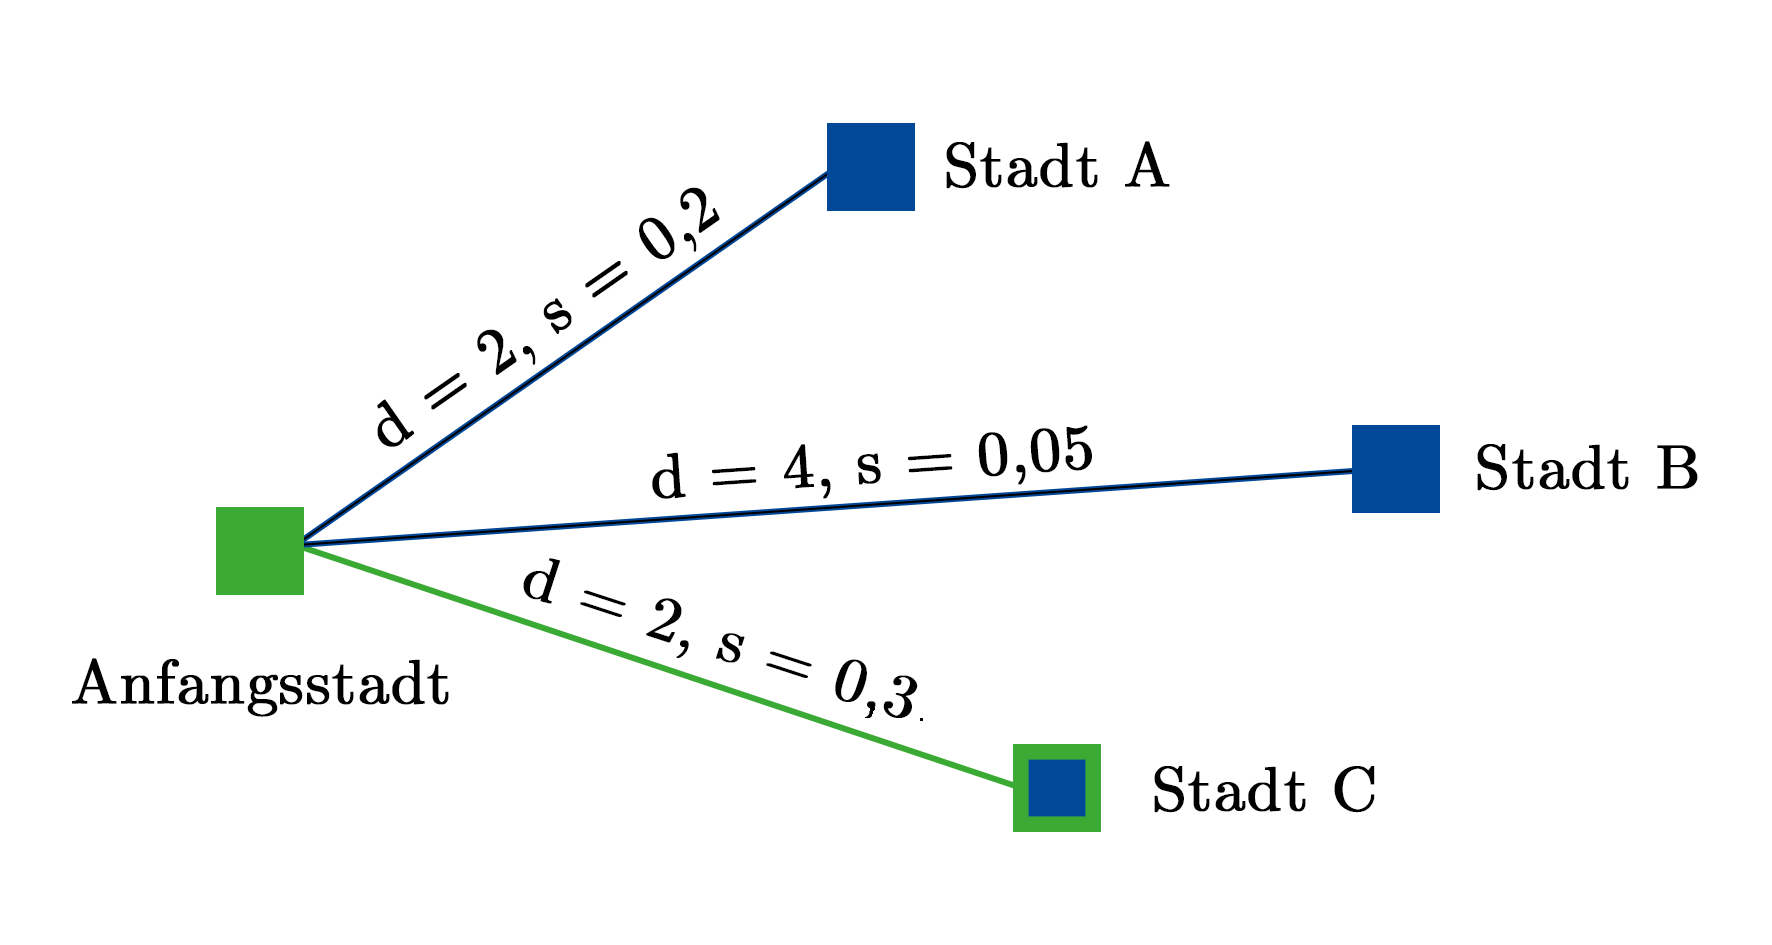
\includegraphics[width=0.8\textwidth]{images/probimage.png}
  \caption[Beispiel für den implementierten Wahrscheinlichkeitsalgorithmus]{Beispiel für den implementierten Wahrscheinlichkeitsalgorithmus. Die Ameise $m$ ermittelt anhand der Parameter $\alpha = 0,9$ und $\beta = 0,3$ und der gegebenen Daten für $d$ und $s$ die jeweilige Wahrscheinlichkeit $p$ und reist dann in die Stadt mit dem höchsten Wert für $p$; in diesem Fall die Stadt C. Dabei wurde die Formel \ref{eq:ProbSimple} für die Berechnung verwendet.}
  \label{img:probimage}
\end{figure}
\\Die Ameise $m$ befindet sich in der als \textit{Anfangsstadt} bezeichneten Stadt. Sie hat nun die Möglichkeit, in eine von drei Städten zu reisen. Als nächstes ermittelt sie nun die Besuchswahrscheinlichkeiten von allen drei Städten. Dazu dienen die Angaben $d$ für die Distanz und $s$ für den Pheromonwert als Grundlage. \\\\Wird ein Parameter Alpha $\alpha$ von $0,9$ und ein Parameter Beta $\beta$ mit $0,3$ gewählt, ergeben sich durch die Nutzung von Formel \ref{eq:ProbSimple} folgende Wahrscheinlichkeiten $p_i$:
\begin{align}
\label{examplePheromone}
p_{Stadt A} = [\tau_{ij}]^\alpha \, [\rfrac{1}{\eta_{ij}}]^\beta = 0,2^{0,9} \cdot (\rfrac{1}{2})^{0,3} = 0,191 \nonumber
\\p_{Stadt B} = [\tau_{ij}]^\alpha \, [\rfrac{1}{\eta_{ij}}]^\beta = 0,05^{0,9} \cdot (\rfrac{1}{4})^{0,3} = 0,045 \nonumber
\\p_{Stadt C} = [\tau_{ij}]^\alpha \, [\rfrac{1}{\eta_{ij}}]^\beta = 0,3^{0,9} \cdot (\rfrac{1}{2})^{0,3} = 0,356 \nonumber
\end{align}
Die Ameise reist nun in die Stadt, welche den größten Wert für $p$ besitzt, dies ist in unserem Beispiel die Stadt C mit $p_{Stadt C} = 0,356$.
\begin{algorithm}
\caption{Ermittlung der nächsten Stadt während der Tourkonstruktion einer Ameise}
\label{probabilityAlg}
\textbf{Eingabe:} Datenobjekt mit $v$ Städten sowie einer Distanzmatrix $D$ und Pheromonmatrix $S$, Ameise $m \in M$ mit einem \texttt{vector} $B$ der Indizes aller schon besuchten Städte, Index $v_k$ der aktuellen Stadt
\\\textbf{Ausgabe:} Index der nächstbesten Stadt $v_{opt}$
\begin{algorithmic}[1]
\State $v_{opt} := -1$
\State $P$ := $\{p_0, ..., p_n\}$ mit $n = v$ 
\For{\textbf{each} Stadt $v_i$ in V}
\If{$v_i \not\in B$ and $v_i \neq v_k$}
\State $p_i$ den Rückgabewert der Wahrscheinlichkeitsformel \ref{eq:Prob} bzw. \ref{eq:ProbSimple} zuweisen
\Else 
\State $p_i := 0$
\EndIf
\EndFor
\State $v_{opt}$ := $v_i$ mit $max(p_i \in P)$
\end{algorithmic}
\end{algorithm}
\subsection{Tourkonstruktionsalgorithmen}
\label{sec:Tourkonstruktionsalgorithmen}
Nachdem mit der Erklärung des Wahrscheinlichkeitsalgorithmus eine wichtige Grundlage für die weitere Implementierung des ACO gelegt wurde, wird nun näher auf die drei implementierten Algorithmen zur Tourkonstruktion eingegangen.
\subsubsection{Iterative Tourkonstruktion}
Bei der ersten implementierten Methode (Algorithmus \ref{IterativeTour}) wird die Pheromonaktualisierung iterativ nach jeder erfolgreichen Tourkonstruktion einer Ameise $m$ vorgenommen. Die nachfolgenden Ameisen können somit für ihre Tourkonstruktion schon die aktualisierten Pheromondaten der vorangegangenen Ameisen nutzen. Der Algorithmus beinhaltet folgende Abbruchbedingung: Wurde in $n$ Iterationen keine kürzere Route gefunden, bricht der Algorithmus ab. Diese Iterationsschwelle $n$ wird dem Algorithmus als Parameter übergeben. Vor dem Beginn der Tourkonstruktion wird zum einen eine Hilfsvariable $j$ definiert, welche für die derzeitige Iteration steht. Sie wird mit $0$ initialisiert. Zum anderen wird die insgesamt kürzeste gefundene Routenlänge $d_s$ mit $\infty$ initialisiert. 
\\Dann startet die Tourkonstruktion. Jede Ameise $m \in M$ startet zunächst in einer zufällig ausgewählten Stadt $v_0$. Diese Stadt stellt auch die erste Stadt $r_{m_0}$ der Route $r$ dar. An dieser Stelle wird eine zweite Hilfsvariable $b$ hinzugefügt, welche die Anzahl der besuchten Städte zählt. Solange diese Variable $b$ nicht der Anzahl der Städte $v$ entspricht, wird die Tour iterativ konstruiert. Welche Stadt $v_b$ dabei als nächstes besucht wird, ergibt sich aus dem oben vorgestellten Wahrscheinlichkeitsalgorithmus. Jeder Index einer besuchten Stadt $v_b$ wird in einen Routenvector $r$ geschrieben; die Distanz $d_m$ wird beim Erreichen einer neuen Stadt mit der Länge der bereisten Kante erweitert und die Zählvariable $b$ wird um $1$ erhöht. Hat eine Ameise alle Städte besucht ($b = |V|$), wird die Tourlänge mit der Distanz von der letzten Stadt $r_{m_b}$ zur ersten Stadt $r_{m_0}$ erweitert. Nun wird die gefundene Routenlänge $d_m$ mit der insgesamt kürzesten Routenlänge $d_s$ verglichen. Ist $d_m$ kleiner als $d_s$, wird $d_s$ mit $d_m$ ersetzt und der Wert der derzeitigen Iteration $j$ wird wieder auf $0$ gesetzt. Abschließend aktualisiert die Ameise $m$ die Pheromonmatrix $S$ und der Iterationszähler $j$ wird um $1$ erhöht. Hat eine Ameise ihre Tourkonstruktion abgeschlossen, startet die nächste Ameise ihre Tour.
\\Der gesamte Algorithmus endet, wenn alle Ameisen in $M$ ihre Tour beendet haben oder wenn nach  $n$ Iterationen keine kürzere Route mehr gefunden wurde. 
\begin{algorithm}
\caption{Iterative Tourkonstruktion}
\label{IterativeTour}
\textbf{Eingabe:} Datenobjekt mit einer Menge $V$ von Städten sowie einer Distanzmatrix $D$ und Pheromonmatrix $S$, \texttt{vector} $M$ mit $m$ Ameisen, Iterationsschwelle $n$
\\\textbf{Ausgabe:} Route $r$ mit der kürzesten gefundenen Distanz $d_s$
\begin{algorithmic}[1]
\State $j := 0$ (derzeitige Iteration, nachdem das letzte Mal eine kürzere Route gefunden wurde)
\State $d_s := \infty$ (kürzeste gefundene Routenlänge)
\For{\textbf{each} Ameise $m \in M$}
\If {$j \leq n$}
\State Starte in einer zufälligen Stadt $v_0$
\State $r_{m_0} := v_0$
\State $b := 1$ (Anzahl der besuchten Städte)
\While{$b \neq |V|$}
\State Ermittle die nächste Stadt $v_b$ und gehe dorthin
\State $r_{m_b} := v_b$
\State $d_m := d_m + D_{r_{m_{b-1}},r_{m_b}}$
\State $b := b + 1$
\EndWhile
\State $d_m := d_m + D_{r_{m_b},r_{m_0}}$
\If{$d_m \leq d_s$}
\State $d_s := d_m$
\State $j := 0$
\EndIf
\State Aktualisiere Pheromonmatrix $S$
\State $j := j + 1$
\EndIf
\EndFor
\end{algorithmic}
\end{algorithm}
\subsubsection{Iterative Tourkonstruktion mit eingeschränkter Pheromonaktualisierung}
Die zweite implementierte Methode ist der ersten sehr ähnlich. Auch hier konstruieren alle Ameisen nacheinander iterativ ihre Tour. Jedoch wird die Pheromonmatrix nur durch die Ameise aktualisiert, welche die kürzeste Route gefunden hat. Diese Vorgehensweise basiert auf dem \textit{Max-Min-Ant-System} von Thomas Stützle und Holger H. Hoos \cite{MaxMin}. Die gesamte Tourkonstruktion erfolgt bei diesem Algorithmus notwendigerweise mehrmals. 
\\Wie bei obigem Algorithmus der normalen iterativen Tourkonstruktion wird auch hier eine Hilfsvariable $j$ mit $0$ initialisiert, welche im weiteren Verlauf des Algorithmus für die aktuelle Iteration steht. Weiterhin wird die Variable $d_s$ für die kürzeste gefundene Distanz mit $\infty$ initalisiert. Zusätzlich wird eine Variable $m_{opt}$ eingeführt, welche den Index der Ameise mit der kürzesten Route jedes Iterationsschritts enthält. Dieser wird zunächst der Wert $-1$ zugewiesen.
\\Bei der nun beginnenden Tourkonstruktion konstruieren alle Ameisen $m \in M$ iterativ ihre Tour. Jede Ameise beginnt in einer Stadt $v_0$. Diese Stadt ist gleichzeitig auch die erste Stadt der Route $r$. Ein Zählvariable $b$ zählt die Anzahl der besuchten Städte. Solange $b \neq |V|$ gilt, also die jeweilige Ameise nicht alle Städte $v$ besucht hat, ermittelt sie die nächste Stadt $v_b$. Die Bestimmung der jeweils nächsten Stadt erfolgt mit dem oben vorgestellten Wahrscheinlichkeitsalgorithmus (siehe Algorithmus \ref{probabilityAlg}). Nach der Reise in die nächste Stadt wird der Zähler $b$ um $1$ inkrementiert und die bisherige Routenlänge $d_m$ entsprechend erhöht.
\\Hat eine Ameise alle Städte besucht, reist sie wieder in ihre Anfangsstadt zurück und die damit bereiste Kante wird zur Routenlänge $d_m$ addiert. Abschließend wird $d_m$ mit der insgesamt kürzesten Routenlänge $d_s$ verglichen. Wurde mit $d_m$ eine kürzere Tour gefunden, so wird $d_s$ durch diese ersetzt und $m_{opt}$ enthält den Index dieser Ameise. 
\\Wurden alle Touren in dem betreffenden Iterationsschritt konstruiert, aktualisiert die Ameise $m_{opt}$ die Pheromonmatrix $S$ und der Iterationszähler $j$ wird um $1$ erhöht. 
\\Dieser gesamte Vorgang wird $n$-mal wiederholt, d. h. solange $j \leq n$ gilt. Die Iterationsschwelle $n$ wird vor dem Start des Programms festgelegt. 
\begin{algorithm}
\caption{Iterative Tourkonstruktion mit eingeschränkter Pheromonaktualisierung}
\label{MMASIterativeTour}
\textbf{Eingabe:} Datenobjekt mit $v$ Städten sowie einer Distanzmatrix $D$ und Pheromonmatrix $S$, \texttt{vector} $M$ mit $m$ Ameisen, Iterationsanzahl $n$
\\\textbf{Ausgabe:} Route $r$ mit der kürzesten gefundenen Distanz $d_s$
\begin{algorithmic}[1]
\State $j := 0$ (derzeitige Iteration)
\State $d_s := \infty$ (kürzeste gefundene Routenlänge)
\State $m_{opt} := -1$ (Index der Ameise mit der kürzesten Route)
\While{$j \leq n$}
\For{\textbf{each} Ameise $m \in M$}
\State Starte in einer zufälligen Stadt $v_0$
\State $r_{m_0} := v_0$
\State $b := 1$ (Anzahl der besuchten Städte)
\While{$b \neq v$}
\State Ermittle die nächste Stadt $v_b$ und gehe dorthin
\State $r_{m_b} := v_b$
\State $d_m := d_m + D_{r_{m_{b-1}},r_{m_b}}$
\State $b := b + 1$
\EndWhile
\State $d_m := d_m + D_{r_{m_b},r_{m_0}}$
\If{$d_m \leq d_s$}
\State $d_s := d_m$
\State $m_{opt} := m_i$
\EndIf
\EndFor
\State Ameise $m_{opt}$ aktualisiert Pheromonmatrix $S$
\State $j := j + 1$
\EndWhile
\end{algorithmic}
\end{algorithm}
\subsubsection{Parallele Tourkonstruktion}
Bei der dritten in dieser Arbeit betrachteten Methode (Algorithmus \ref{ParallelTour}) konstruieren die Ameisen ihre Route parallel.
Als Erstes wird hierfür eine Hilfsvariable $j$ definiert und mit $0$ initialisiert. Diese dient als Zähler für die aktuell besuchten Städte. Weiterhin wird eine Variable für die kürzeste gefundene Distanz $d_s$ mit $\infty$ initialisiert. \\Dann startet die Tourkonstruktion, die mithilfe einer \texttt{For}-Schleife realisiert wird. Jede Ameise startet in einer zufälligen Stadt $v_0$, die gleichzeitig auch die erste Stadt $r_{m_0}$ der Route ist. Nun ermittelt jede Ameise $m$ zunächst die erste Stadt $v_1$. Die 2. Stadt der Route $r$ einer jeden Ameise $m$ ist nun die Stadt $v_1$. Dann wird die Tourlänge $d_m$ mit der Distanz von der Stadt $v_0$ zur Stadt $v_1$ verlängert. Abschließend aktualisiert jede Ameise die Pheromonkonzentration auf der begangenen Kante und der Zähler $j$ wird um $1$ erhöht.
\\Dieses Vorgehen geschieht analog für jede weitere Stadt $v_j$. Wenn jede Ameise jede Stadt einmal besucht hat, endet der Algorithmus. Abschließend wird ein weiteres Mal durch die Menge $M$ der Ameisen iteriert, um zunächst die Tourlänge um die Distanz von der letzten Stadt $r_{m_j}$ zur ersten Stadt $r_{m_0}$ zu erweitern. Die insgesamt kürzeste Route $d_s$ ergibt sich abschließend durch den Vergleich der Routenlängen aller Ameisen.
\begin{algorithm}
\caption{Parallele Tourkonstruktion}
\label{ParallelTour}
\textbf{Eingabe:} Datenobjekt mit $v$ Städten sowie einer Distanzmatrix $D$ und Pheromonmatrix $S$, \texttt{vector} $M$ mit $m$ Ameisen
\\\textbf{Ausgabe:} Route $r$ mit der kürzesten gefundenen Distanz $d_s$
\begin{algorithmic}[1]
\State $j := 0$
\State $d_s = \infty$
\While{$j < v$}
\For{\textbf{each} Ameise $m \in M$}
\If{$j = 0$}
\State $r_{m_0} := v_0$
\EndIf
\State Starte in einer zufälligen Stadt $v_0$
\State Ermittle die nächste Stadt $v_j$ und gehe dorthin
\State $r_{m_j} := v_j$
\hspace{17em}\raisebox{1.3\baselineskip}[0pt][0pt]{$\left.\rule{0pt}{3.8\baselineskip}\right\}\ \mbox{parallel}$}
\State $d_m := d_m + D_{r_{m_{j-1}},r_{m_j}}$
\State Aktualisiere Pheromonmatrix $S$
\EndFor
\State $j := j + 1$
\EndWhile
\For{\textbf{each} Ameise $m \in M$} 
\State $d_m := d_m + D_{r_{m_j},r_{m_0}}$
\If{Tourlänge $d_m < d_s$}
\State $d_s := d_m$
\EndIf
\EndFor
\end{algorithmic}
\end{algorithm}
\newpage\section{Experimente}
\label{sec:vorgehensweise}
Im Rahmen dieser Arbeit werden zur Untersuchung der oben vorgestellten Algorithmen zur Lösung des TSP der TSPLIB vier symmetrische Probleminstanzen entnommen: \texttt{burma14}, \texttt{dantzig42}, \texttt{gr120} und \texttt{si535}. Nähere Informationen zu diesen Instanzen finden sich in Tabelle \ref{tsplibdesc}.
\begin{table}[]
\centering
\resizebox{\textwidth}{!}{%
\begin{tabular}{@{}llll@{}}
\toprule
\multicolumn{1}{c|}{Probleminstanz} & \multicolumn{1}{c}{Anzahl der Städte} & \multicolumn{1}{c}{optimale Tourlänge} &Beschreibung   \\ \midrule
\multicolumn{1}{l|}{burma14}        & 14                                    & 3323                                   & geographisches Problem             \\
\multicolumn{1}{l|}{dantzig42}      & 42                                    & 699                                    & geographisches Problem             \\
\multicolumn{1}{l|}{gr120}          & 120                                   & 6942                                   & geographisches Problem             \\
\multicolumn{1}{l|}{si535}          & 535                                   & 48450                                  & fiktives Problem von M. Hofmeister \\ \bottomrule
\multicolumn{4}{l}{}                                                                                                                                     
\end{tabular}%
}
\caption{Übersicht über die untersuchten TSPLIB-Instanzen mit den Angaben zur Anzahl der Städte, zum Tourlängenoptimum und zur Art des Problems}
\label{tsplibdesc}
\end{table}
\\Die unterschiedlichen Größen der gewählten Instanzen dienen einer besseren Beurteilung der Effektivität und Laufzeit des Programms.
Der Begriff \textit{Effektivität} bezieht sich dabei im Folgenden immer auf die Eigenschaft, in Bezug auf die Tourlänge möglichst nah an das Optimum heranzukommen. Sowohl die Laufzeit als auch die Effektivität hängen von mehreren Parametern ab:
\begin{itemize}
\item[$\alpha$:] legt die Wichtigkeit der Pheromonkonzentration auf einer Kante bei der Wahl der nächsten zu bereisenden Stadt fest
\item[$\beta$:] bestimmt die Wichtigkeit der Distanz auf einer Kante bei der Wahl der nächsten zu bereisenden Stadt 
\item[$Q$:] stellt die Menge des abgelegten Pheromons dar
\item[$\rho$:] gibt den Wert der Pheromonpersistenz an; $1 - \rho$ steht für die Pheromonverdunstung
\end{itemize}
Zunächst werden deshalb anhand der \texttt{dantzig42}-Instanz die Auswirkungen der oben genannten Parameter betrachtet und die Ergebnisse für verschiedene Werte erfasst.
Dies geschieht für alle drei umgesetzten Algorithmen unter Berücksichtigung der verschiedenen Implementierungen für die Wahrscheinlichkeitsermittlung der nächsten Stadt bei der Tourkonstruktion (Abschnitt \ref{structure}.).
Die dadurch gewonnenen Werte für die Parameter werden hinsichtlich der Effektivität verglichen. 
\\\\Die Untersuchung der implementierten Algorithmen und des Einflusses der einzelnen Parameter wird auf einem Rechner mit einem AMD Athlon II 3800 Mhz QuadCore-Prozessor und 8 Gigabyte DDR3 RAM durchgeführt. Das Betriebssystem ist dabei Microsoft Windows 10 in der Home-Edition.
\\Zur besseren Analysemöglichkeit werden alle Daten in eine CSV-Datei geschrieben und von dort aus mit Microsoft Excel ausgewertet.
\\Um die Laufzeit eines Problems zu messen, wird die C\texttt{++}-Bibliothek \texttt{chrono} verwendet. Dabei wird die Systemzeit bei Beginn und Ende der Routenberechnung gemessen. Die Laufzeit ergibt sich dann aus der Differenz beider Werte. 
\\Die Effektivität ergibt sich aus der Abweichung vom Tourlängen-Optimum. Dabei werden der maximale bzw. minimale Abstand und der Durchschnitt in mehreren Programmdurchläufen erfasst und prozentual ermittelt.
\\Für alle nachfolgenden Experimente wurde die Pheromonkonzentration auf allen Kanten mit dem Wert $0,01$ initialisiert.
\subsection{Einfluss der Parameter auf die implementierten Algorithmen}
\label{sec:einflussparameter}
In diesem Abschnitt wird zunächst der Einfluss der in Abschnitt \ref{sec:vorgehensweise} besprochenen wesentlichen Parameter diskutiert und grafisch dargestellt. 
\subsubsection{Parametereinfluss auf den iterativen Algorithmus}
Der iterative Algorithmus ist die klassische Umsetzung zur Lösung einer TSP-Probleminstanz mit dem Ameisenalgorithmus. Deswegen wird dieser unter dem Einfluss der einzelnen Parameter zuerst betrachtet. \\Bei der Untersuchung wurden zunächst die Parameter Alpha $\alpha$ und Beta $\beta$ für das Intervall $0,05 \leq \{\alpha,\beta\} \leq 1$ mit einer Schrittweite von $0,05$ iteriert. Dies wurde mit einer doppelten \texttt{For}-Schleife umgesetzt:
\begin{lstlisting}
for (double alpha = 0,05; alpha <= 1,0; alpha += 0,05)
	for (double beta = 0,05; beta <= 1,0; beta += 0,05) 
		RunAlgorithm();
\end{lstlisting}
Somit ergibt sich für jeden Wert von Alpha $\alpha$ die Abhängigkeit von allen Werten für Beta $\beta$ und umgekehrt. Die Werte für die Pheromonablagemenge und die Pheromonpersistenz wurden auf $Q = 40$ und $\rho = 0,25$ festgelegt.
\\Die gleiche Vorgehensweise wurde analog für die Parameter $Q$ (Menge des abgelegten Pheromons) und $\rho$ (Pheromonpersistenz) durchgeführt.
Hierbei wurde für $Q$ das Intervall $2 \leq Q \leq 42$ mit einer Schrittweite von $2$ und für $\rho$ das Intervall $0,05 \leq \rho \leq 0,95$ mit einer Schrittweite von $0,05$ gewählt. Die Werte für Alpha $\alpha$ und Beta $\beta$ sind konstant mit $\alpha = 1$ und $\beta = 0,25$. 
\begin{lstlisting}
for (double q = 2; q <= 42; q += 2)
	for (double rho = 0,05; rho <= 0,95; rho += 0,05) 
		RunAlgorithm();
\end{lstlisting}
Eine Übersicht aller Parameterwerte mit den entsprechenden Intervallen und Schrittweiten ist in Tabelle \ref{tableiterativvalues} ersichtlich.
\begin{table}[]
\centering
\resizebox{\textwidth}{!}{%
\begin{tabular}{@{}llll@{}}
\toprule
\multicolumn{1}{l|}{Parameter}                 & Intervall                  & Schrittweite & Parameterwert bei Untersuchung der anderen Parameter \\ \midrule
\multicolumn{1}{l|}{Alpha $\alpha$}            & $0,05 \leq \alpha \leq 1$  & 0,05         & 1                                                    \\
\multicolumn{1}{l|}{Beta $\beta$}              & $0,05 \leq \beta \leq 1$   & 0,05         & 0,25                                                 \\
\multicolumn{1}{l|}{Pheromonablagemenge $Q$}   & $2 \leq Q \leq 42$         & 2            & 40                                                   \\
\multicolumn{1}{l|}{Pheromonpersistenz $\rho$} & $0,05 \leq \rho \leq 0,95$ & 0,05         & 0,25                                                 \\ \bottomrule
\multicolumn{4}{l}{}                                                                                                                             
\end{tabular}%
}
\caption[Übersicht über die Parameterwerte für die Untersuchung der Abhängigkeit der Tourlänge von den einzelnen Parameter bei Betrachtung des iterativen Algorithmus zur Tourkonstruktion]{Übersicht über die Parameterwerte für die Untersuchung der Abhängigkeit der einzelnen Parameter bei Betrachtung des iterativen Algorithmus zur Tourkonstruktion. Die Spalte \glqq Parameterwert bei Untersuchung der anderen Parameter\grqq\, gibt an, welche Werte für Alpha $\alpha$ und Beta $\beta$ bei Untersuchung der Pheromonablagemenge und der Pheromonpersistenz gewählt wurden und umgekehrt.}
\label{tableiterativvalues}
\end{table}
\\Die Ergebnisse finden sich grafisch dargestellt in Abbildung \ref{fig:iterativeDiagram}. Dabei ist die Tourlänge in Abhängigkeit von allen vier Parametern dargestellt. Die verschiedenen Tourlängen für jeden Wert eines Parameters ergeben sich durch unterschiedliche Werte für den jeweils anderen Parameter, der zusammen mit diesem untersucht wurde. Diese Art der Erfassung der Parameterwerte wurde als ausreichend erachtet und auf eine mehrmalige Durchführung dieser Tests wurde aufgrund der Menge der Daten verzichtet. Der Durchschnitt dieser Werte wird durch den Funktionsgraph dargestellt. 
\\\\Es lässt sich deutlich erkennen, dass sowohl der Parameter $\alpha$, der über die Wichtigkeit der Pheromonspur Auskunft gibt, als auch der Parameter $Q$, der die abgelegte Pheromonmenge darstellt, bei Veränderung im gewählten Wertebereich keinen großen Einfluss auf die Tourlängen haben. Mit einem steigenden Einfluss von Parameter $\beta$ werden die Routen insgesamt kürzer. Am meisten beeinflusst jedoch der Parameter $\rho$ für die Pheromonpersistenz die gefundenen Tourlängen. Je mehr sich dieser Parameter dem Wert $1$ nähert, umso kürzer werden die Routen im Durchschnitt.
\begin{figure}
        \centering
        \captionsetup[subfigure]{oneside,margin={0.5cm,0cm}}
        \begin{subfigure}[b]{0.475\textwidth}
            \centering
            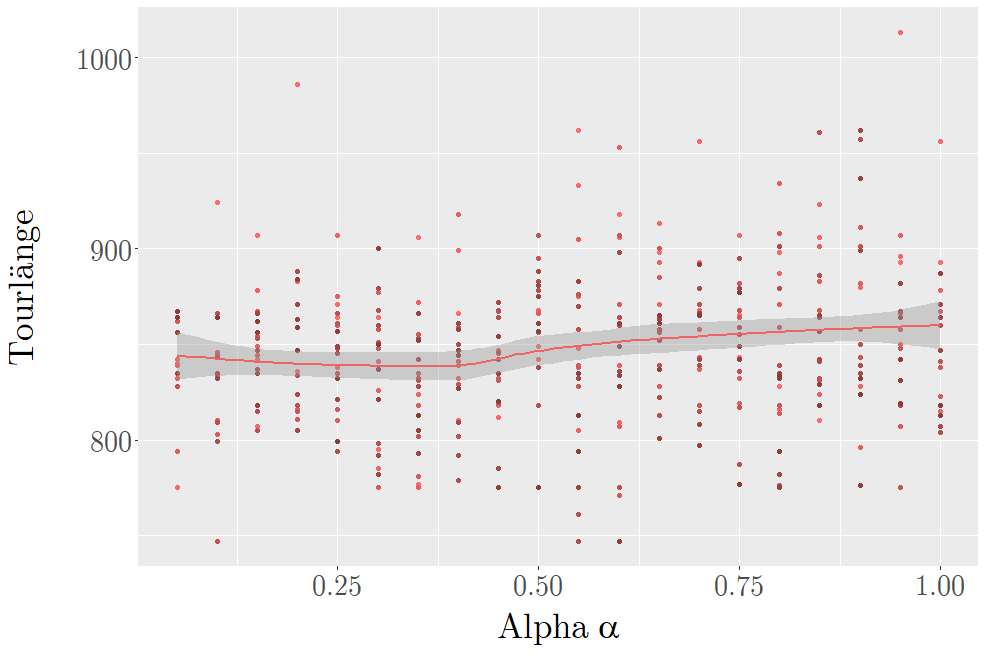
\includegraphics[width=\textwidth]{images/diagramiterativealpha}
            \caption{Alpha $\alpha$ mit verschiedenen Werten für Beta $\beta$}               
            \label{fig:iterativeAlpha}
        \end{subfigure}
        \hfill
        \begin{subfigure}[b]{0.475\textwidth}  
            \centering 
            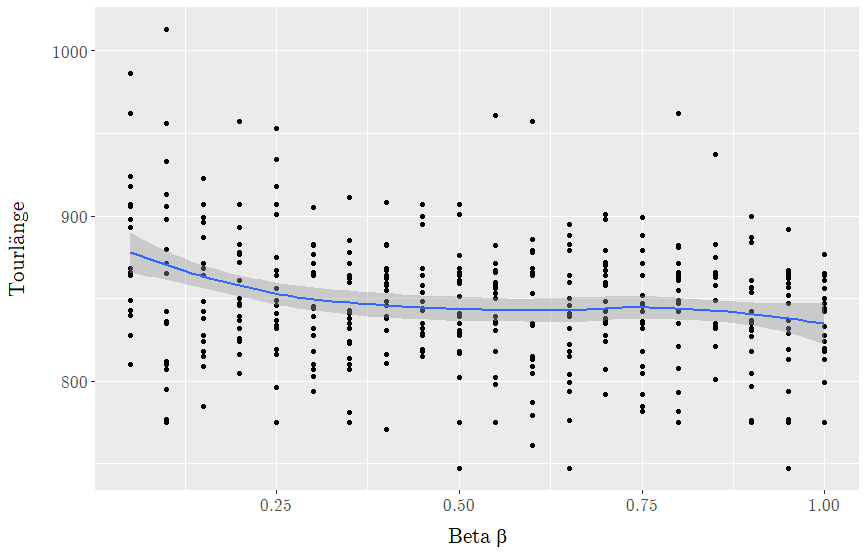
\includegraphics[width=\textwidth]{images/diagramiterativebeta}
            \caption{Beta $\beta$ mit verschiedenen Werten für Alpha $\alpha$}   
            \label{fig:iterativeBeta}
        \end{subfigure}
        \vskip\baselineskip
        \begin{subfigure}[b]{0.475\textwidth}   
            \centering 
            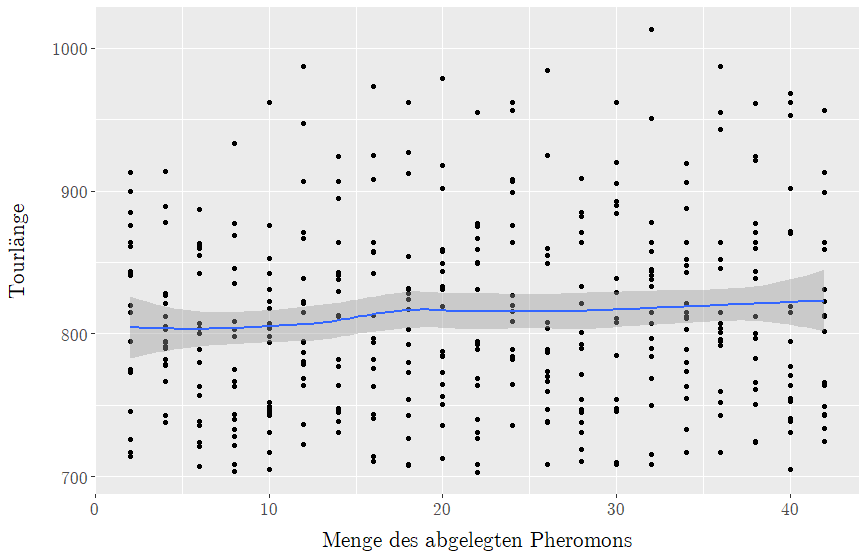
\includegraphics[width=\textwidth]{images/diagramiterativedeposit}
            \caption{Menge des abgelegten Pheromons mit verschiedenen Werten für die Pheromonpersistenz}   
            \label{fig:iterativeDeposit}
        \end{subfigure}
        \quad
        \begin{subfigure}[b]{0.475\textwidth}   
            \centering 
            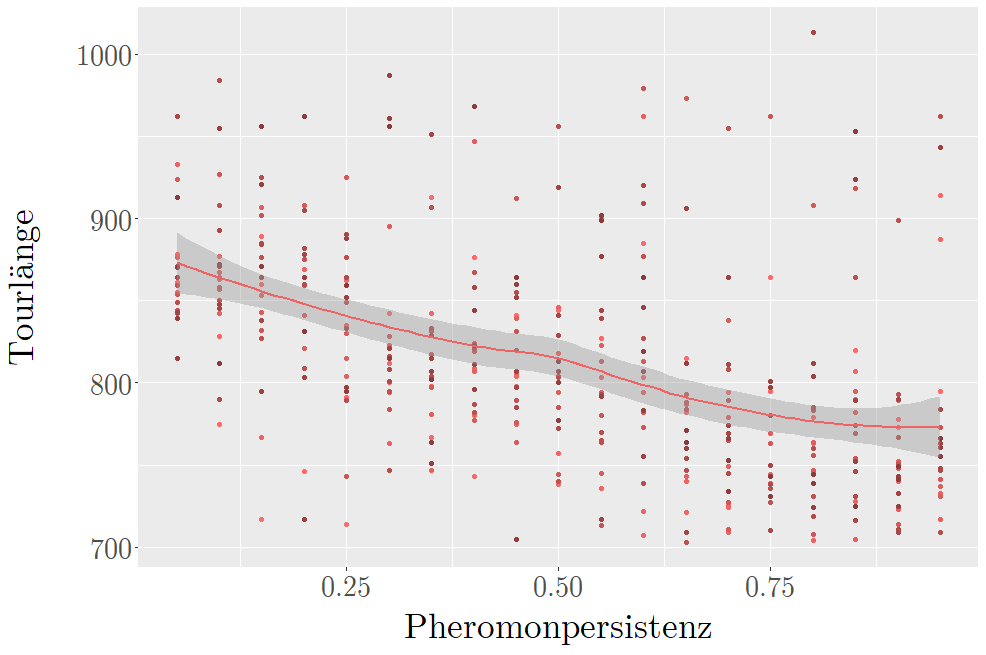
\includegraphics[width=\textwidth]{images/diagramiterativereduction}
            \caption{Pheromonpersistenz mit verschiedenen Werten für die Pheromonablagemenge}   
            \label{fig:iterativeReduction}
        \end{subfigure}
        \caption{Abhängigkeit der Tourlänge von den einzelnen Parametern bei der iterativen Tourkonstruktion } 
        \label{fig:iterativeDiagram}
    \end{figure}
\subsubsection{Parametereinfluss auf den iterativen Algorithmus mit eingeschränkter Pheromonaktualisierung}
Wie bei dem oben untersuchten iterativen Algorithmus wurden auch hier die Parameter Alpha $\alpha$ und Beta $\beta$ sowie $Q$ und $\rho$ kombiniert untersucht. Dazu wurde, wie schon oben gezeigt, jeweils eine doppelte \texttt{For}-Schleife verwendet. Auch hier ergeben sich die verschiedenen Tourlängen für jeden Wert eines Parameters durch unterschiedliche Werte für den jeweils mituntersuchten Parameter. Aufgrund der höheren Komplexität und damit einer höheren Laufzeit wurden die Schrittweiten zwischen den einzelnen Werten doppelt so groß wie ber vorherigen Untersuchung gewählt. Der Wertebereich für die einzelnen Parameter ist für Alpha $\alpha$ und Beta $\beta$ derselbe; für die Pheromonablagemenge wurde ein Wertebereich von $2 \leq Q \leq 46$, für die Pheromonpersistenz ein Wertebereich von $0,1 \leq \rho \leq 1$ gewählt. Die genauen Werte finden sich in Tabelle \ref{tablemmasvalues} als Übersicht wieder.
\begin{table}[]
\centering
\resizebox{\textwidth}{!}{%
\begin{tabular}{@{}llll@{}}
\toprule
\multicolumn{1}{l|}{Parameter}                 & Intervall                  & Schrittweite & Parameterwert bei Untersuchung der anderen Parameter \\ \midrule
\multicolumn{1}{l|}{Alpha $\alpha$}            & $0,05 \leq \alpha \leq 1$  & 0,05         & 1                                                    \\
\multicolumn{1}{l|}{Beta $\beta$}              & $0,05 \leq \beta \leq 1$   & 0,05         & 0,25                                                 \\
\multicolumn{1}{l|}{Pheromonablagemenge $Q$}   & $2 \leq Q \leq 42$         & 2            & 40                                                   \\
\multicolumn{1}{l|}{Pheromonpersistenz $\rho$} & $0,05 \leq \rho \leq 0,95$ & 0,05         & 0,25                                                 \\ \bottomrule
\multicolumn{4}{l}{}                                                                                                                             
\end{tabular}%
}
\caption[Übersicht über die Parameterwerte für die Untersuchung der Abhängigkeit der einzelnen Parameter bei Betrachtung des iterativen Algorithmus mit eingeschränkter Pheromonaktualisierung zur Tourkonstruktion]{Übersicht über die Parameterwerte für die Untersuchung der Abhängigkeit der Tourlänge von den einzelnen Parameter bei Betrachtung des iterativen Algorithmus mit eingeschränkter Pheromonaktualisierung zur Tourkonstruktion. Die Spalte \glqq Parameterwert bei Untersuchung der anderen Parameter\grqq\, gibt an, welche Werte für Alpha $\alpha$ und Beta $\beta$ bei Untersuchung der Pheromonablagemenge und der Pheromonpersistenz gewählt wurden und umgekehrt.}
\label{tablemmasvalues}
\end{table}
\\Der Algorithmus lässt vom Namen her auf eine ähnliche Tourlängenbeeinflussung durch die Parameter wie der iterative Algorithmus schließen. Jedoch gestaltet sich der Parametereinfluss wesentlich anders. Dies geht aus Abbildung \ref{fig:mmasDiagram} hervor. 
\begin{figure}[!]
        \centering
        \captionsetup[subfigure]{oneside,margin={0.5cm,0cm}}
        \begin{subfigure}[b]{0.475\textwidth}
            \centering
            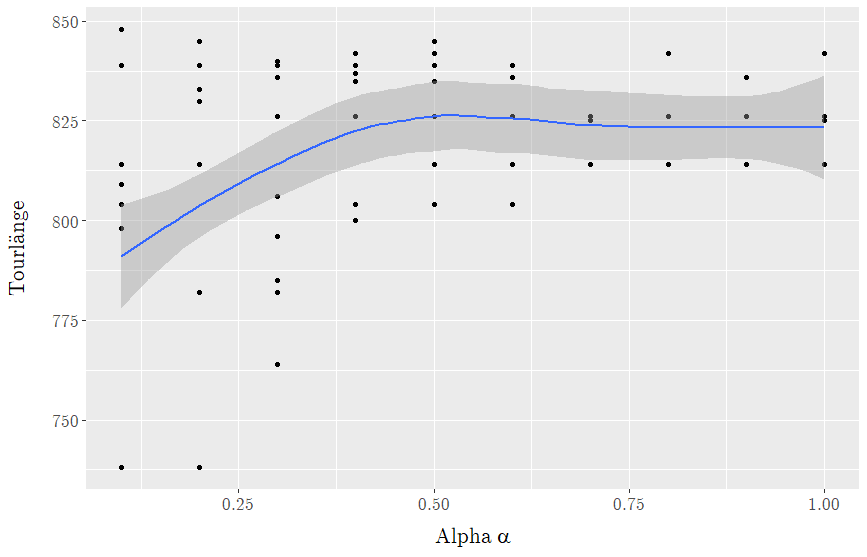
\includegraphics[width=\textwidth]{images/diagrammmasalpha}
            \caption{Alpha $\alpha$ mit verschiedenen Werten für Beta $\beta$}               
            \label{fig:iterativeAlpha}
        \end{subfigure}
        \hfill
        \begin{subfigure}[b]{0.475\textwidth}  
            \centering 
            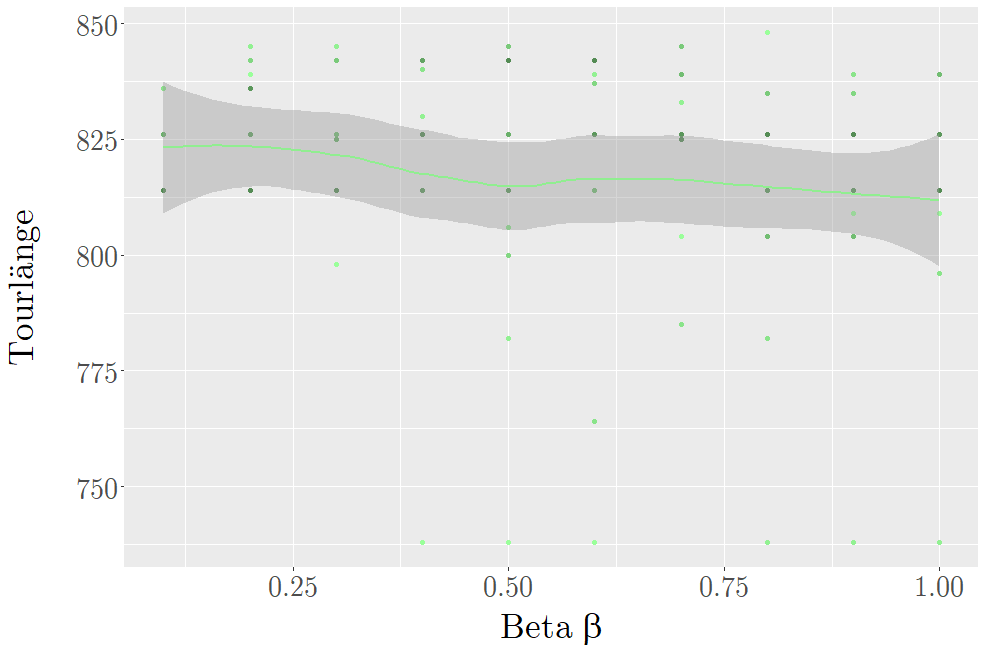
\includegraphics[width=\textwidth]{images/diagrammmasbeta}
            \caption{Beta $\beta$ mit verschiedenen Werten für Alpha $\alpha$}   
            \label{fig:iterativeBeta}
        \end{subfigure}
        \vskip\baselineskip
        \begin{subfigure}[b]{0.475\textwidth}   
            \centering 
            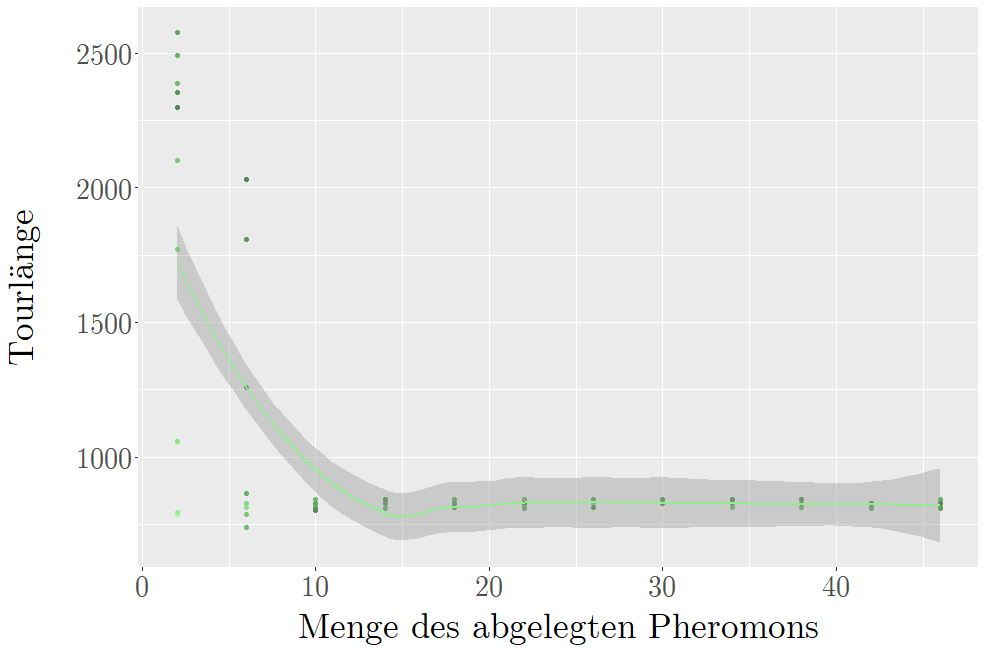
\includegraphics[width=\textwidth]{images/diagrammmasdeposit}
            \caption{Menge des abgelegten Pheromons mit verschiedenen Werten für die Pheromonpersistenz}   
            \label{fig:iterativeDeposit}
        \end{subfigure}
        \quad
        \begin{subfigure}[b]{0.475\textwidth}   
            \centering 
            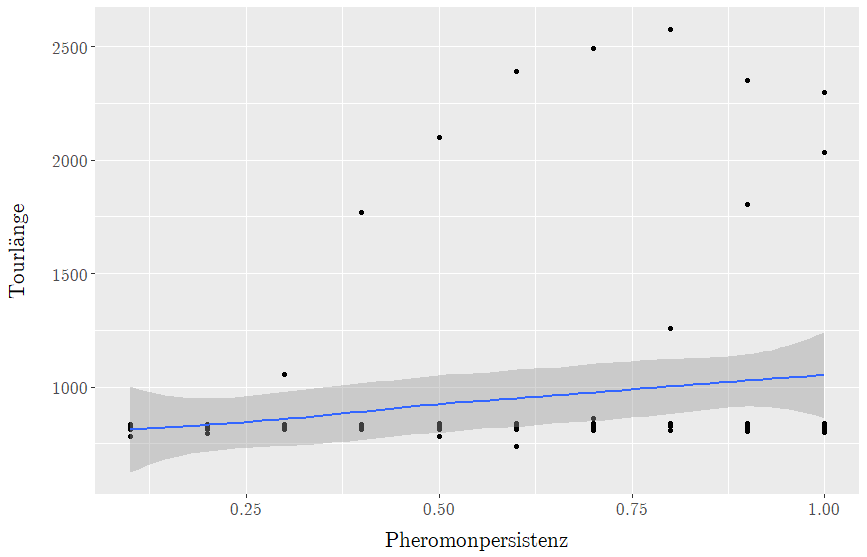
\includegraphics[width=\textwidth]{images/diagrammmasreduction}
            \caption{Pheromonpersistenz mit verschiedenen Werten für die Pheromonablagemenge}   
            \label{fig:iterativeReduction}
        \end{subfigure}
        \caption{Abhängigkeit der Tourlänge von den einzelnen Parametern bei der iterativen Tourkonstruktion mit eingeschränkter Pheromonaktualisierung } 
        \label{fig:mmasDiagram}
    \end{figure}
\\Der Parameter Beta $\beta$, der die Wichtigkeit der Distanz bei der Ermittlung der nächsten Stadt während der Tourkonstruktion angibt, 
lässt das Finden leicht kürzerer Routen bei Annäherung gegen $1$ zu. Der Parameter Alpha $\alpha$ dagegen beeinflusst das Finden kurzer Touren bei Annäherung gegen $1$ eher negativ. Jedoch ist die Streuung bei kleinen Werten für $\alpha$ wesentlich höher. 
\\Die Menge des abgelegten Pheromons erzielt ab einem Wert von $10$ die besten Ergebnisse mit einer sehr geringen Streuung. Für einen Wert von $Q = 2$ erreicht der Algorithmus teilweise Tourlängen mit einer Abweichung von fast $300 \%$ vom Optimum. Die Pheromonpersistenz $\rho$ steigt für höhere Werte leicht an und ist für einen Wert im Bereich von $0,05$ bis $0,10$ im Hinblick auf die Tourlänge und eine geringe Streuung optimal.
\subsubsection{Parametereinfluss auf den parallelen Algorithmus}
Beim dritten und letzten implementierten Algorithmus wird der Parametereinfluss wie bei den zwei vorhergehenden Algorithmen durch Kombination der Parameter untersucht. Auch hier werden Alpha $\alpha$ und Beta $\beta$ zusammen im Intervall von $0,05 \leq \{\alpha,\beta\} \leq 1$ untersucht - jeweils mit einer Schrittweite von $0,05$. Für die Pheromonablage- und Pheromonpersistenzwerte wurde ein Wertebereich von $2 \leq Q \leq 42$ mit einer Schrittweite von $2$ bzw. von $0,05 \leq \rho \leq 0,95$ mit einer Schrittweite von $0,05$ gewählt.
Wie auch oben finden sich diese Werte in einer Tabelle als Übersicht (Tabelle \ref{tableparallelvalues}). Dabei existieren für jeden Parameterwert mehrere Ergebnisse entsprechend der Anzahl aller Werte des Parameters, der in Kombination mit diesem untersucht wurde. 
\begin{table}[]
\centering
\resizebox{\textwidth}{!}{%
\begin{tabular}{@{}llll@{}}
\toprule
\multicolumn{1}{l|}{Parameter}                 & Intervall                  & Schrittweite & Parameterwert bei Untersuchung der anderen Parameter \\ \midrule
\multicolumn{1}{l|}{Alpha $\alpha$}            & $0,05 \leq \alpha \leq 1$  & 0,05         & 1                                                    \\
\multicolumn{1}{l|}{Beta $\beta$}              & $0,05 \leq \beta \leq 1$   & 0,05         & 0,25                                                 \\
\multicolumn{1}{l|}{Pheromonablagemenge $Q$}   & $2 \leq Q \leq 42$         & 2            & 40                                                   \\
\multicolumn{1}{l|}{Pheromonpersistenz $\rho$} & $0,05 \leq \rho \leq 0,95$ & 0,05         & 0,25                                                 \\ \bottomrule
\multicolumn{4}{l}{}                                                                                                                             
\end{tabular}%
}
\caption[Übersicht über die Parameterwerte für die Untersuchung der Abhängigkeit der Tourlänge von den einzelnen Parametenr bei Betrachtung des parallelen Algorithmus zur Tourkonstruktion]{Übersicht über die Parameterwerte für die Untersuchung der Abhängigkeit der Tourlänge von den einzelnen Parametern bei Betrachtung des parallelen Algorithmus zur Tourkonstruktion. Die Spalte \glqq Parameterwert bei Untersuchung der anderen Parameter\grqq\, gibt an, welche Werte für Alpha $\alpha$ und Beta $\beta$ bei Untersuchung der Pheromonablagemenge und der Pheromonpersistenz gewählt wurden und umgekehrt.}
\label{tableparallelvalues}
\end{table}
\\Anhand von Abbildung \ref{fig:parallelDiagram} lässt sich erkennen, dass für Alpha $\alpha$ bessere Tourlängenwerte bei Annäherung gegen $1$ erzielt werden. 
\begin{figure}[!]
        \centering
        \captionsetup[subfigure]{oneside,margin={0.5cm,0cm}}
        \begin{subfigure}[b]{0.475\textwidth}
            \centering
            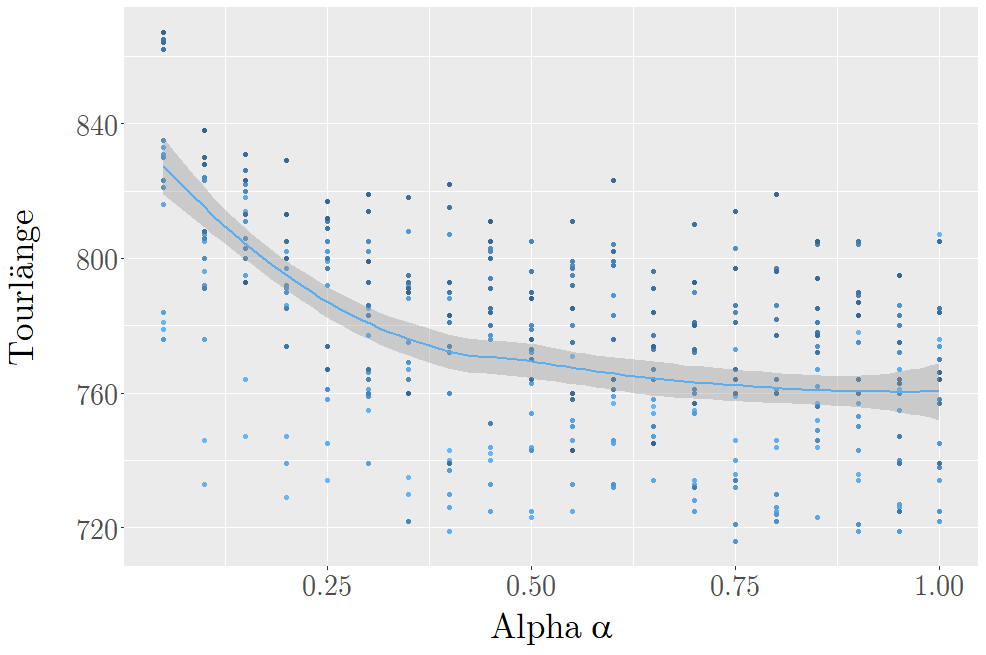
\includegraphics[width=\textwidth]{images/diagramparallelalpha}
            \caption{Alpha $\alpha$ mit verschiedenen Werten für Beta $\beta$}               
            \label{fig:iterativeAlpha}
        \end{subfigure}
        \hfill
        \begin{subfigure}[b]{0.475\textwidth}  
            \centering 
            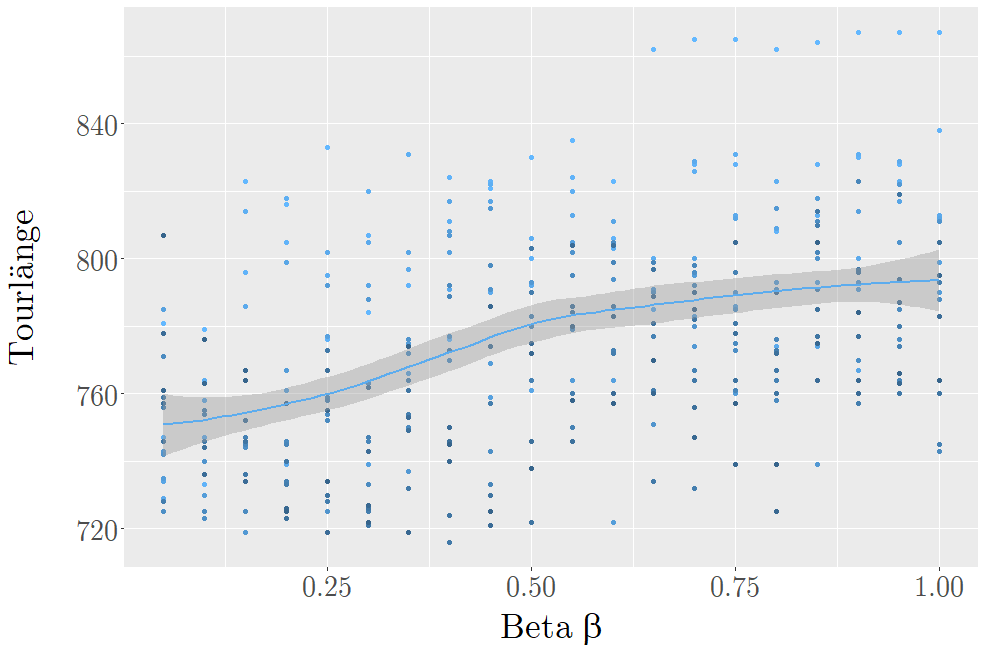
\includegraphics[width=\textwidth]{images/diagramparallelbeta}
            \caption{Beta $\beta$ mit verschiedenen Werten für Alpha $\alpha$}   
            \label{fig:iterativeBeta}
        \end{subfigure}
        \vskip\baselineskip
        \begin{subfigure}[b]{0.475\textwidth}   
            \centering 
            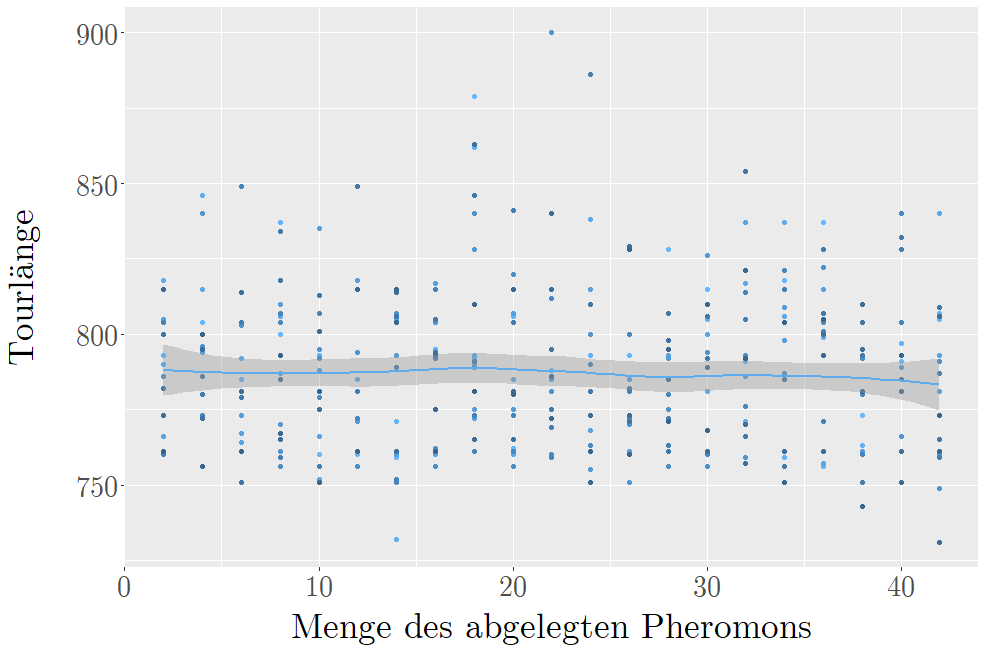
\includegraphics[width=\textwidth]{images/diagramparalleldeposit}
            \caption{Menge des abgelegten Pheromons mit verschiedenen Werten für die Pheromonpersistenz}   
            \label{fig:iterativeDeposit}
        \end{subfigure}
        \quad
        \begin{subfigure}[b]{0.475\textwidth}   
            \centering 
            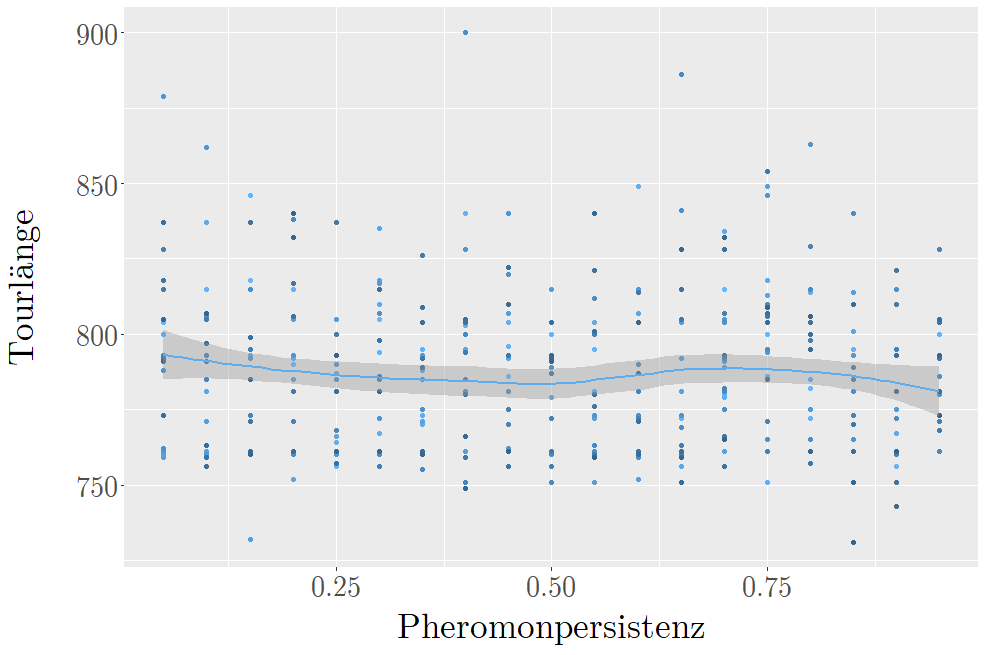
\includegraphics[width=\textwidth]{images/diagramparallelreduction}
            \caption{Pheromonpersistenz mit verschiedenen Werten für die Pheromonablagemenge}   
            \label{fig:iterativeReduction}
        \end{subfigure}
        \caption{Abhängigkeit der Tourlänge von den einzelnen Parametern bei der parallelen Tourkonstruktion } 
        \label{fig:parallelDiagram}
    \end{figure}
Für Beta $\beta$ ist dieser Sachverhalt genau umgekehrt - hier werden die besten Werte bei einem geringen Einfluss der Distanz auf die Tourkonstruktion erzielt. Für die Parameter $Q$ und $\rho$ lässt sich keine große Veränderung der Tourlängen feststellen; die gefundenen Tourlängen sind im Mittel konstant für alle unterschiedlichen Werte.
\newpage
\subsection{Auswirkung des gewählten Wahrscheinlichkeitsalgorithmus}
\label{AuswirkungWA}
Wie schon in Abschnitt \ref{enum:Update}. vorgestellt, wurden für die Erstellung dieser Arbeit zwei verschiedene Formeln zur Ermittlung der Wahrscheinlichkeiten der nächsten Städte bei der Tourkonstruktion implementiert. Zum einen ist dies die Formel \ref{eq:Prob}, die unter anderem von Thomas Stützle und Holger H. Hoos in ihrem vorgestellten \textit{Max-Min-Ant-System} verwendet wurde. Im Folgenden wird der Algorithmus, der diese Formel verwendet, der Einfachheit halber \textit{Komplexer Wahrscheinlichkeitsalgorithmus} genannt. Der andere Wahrscheinlichkeitsalgorithmus verwendet eine vereinfachte Form dieser Formel (Formel \ref{eq:ProbSimple}) und wird im Folgenden als \textit{Einfacher Wahrscheinlichkeitsalgorithmus} bezeichnet.
\\Bei der Untersuchung wurden für die einzelnen Parameter folgende Werte verwendet: $\alpha = 1$, $\beta = 0,25$, $Q = 40$ und $\rho = 0,15$. Für die Erhebung von statistischen Daten wurde jeder Algorithmus zur Tourkonstruktion mit jedem Wahrscheinlichkeitsalgorithmus zehnmal getestet. Die verwendete Probleminstanz war \texttt{dantzig42} mit einem Tourlängenoptimum von $699$.
\newpage
Die Ergebnisse sind in folgender Tabelle dargestellt:
\begin{table}[]
\captionsetup{justification=centering}
\centering
\resizebox{\textwidth}{!}{%
\begin{tabular}{@{}lllllll@{}}
\toprule
 & \multicolumn{6}{c}{Wahrscheinlichkeitsermittlung} \\
 & \multicolumn{3}{c|}{Einfach} & \multicolumn{3}{c}{Komplex} \\
\multicolumn{1}{c|}{Algorithmus} & \begin{tabular}[c]{@{}l@{}}Tourlänge\\ (Durchschnitt)\end{tabular} & {[}\%{]} & \multicolumn{1}{l|}{Zeit in $s$} & \begin{tabular}[c]{@{}l@{}}Tourlänge\\ (Durchschnitt)\end{tabular} & {[}\%{]} & Zeit in $s$ \\ \midrule
\multicolumn{1}{l|}{Iterativ} & 746,3 & 6,77 & \multicolumn{1}{l|}{3,49} & 733,1 & 4,88 & 55,46 \\
\multicolumn{1}{l|}{Iterativ mit eingeschränkter Pheromonaktualisierung} & 849,7 & 21,56 & \multicolumn{1}{l|}{5,13} & 880,5 & 25,97 & 71,23 \\
\multicolumn{1}{l|}{Parallel} & 818 & 17,02 & \multicolumn{1}{l|}{23,33} & 832,6 & 19,11 & 447,45 \\ \bottomrule
\multicolumn{7}{l}{}
\end{tabular}%
}
\caption[Ergebnisse für die einzelnen Algorithmen in Abhängigkeit des gewählten Wahrscheinlichkeitsalgorithmus]{Ergebnisse für die einzelnen Algorithmen in Abhängigkeit des gewählten Wahrscheinlichkeitsalgorithmus. Die Prozentzahl hinter der Tourlänge zeigt die Abweichung vom Tourlängenoptimum $d = 699$ an}
\label{table:Prob}
\end{table}
\\Auffallend ist, dass der komplexe Wahrscheinlichkeitsalgorithmus im Vergleich zu dem einfachen Algorithmus sehr viel mehr Zeit zur Berechnung benötigt. Dieser Unterschied beträgt teilweise bis zu $2000 \,\%$.
Im Hinblick auf die gefundenen Routenlängen lässt  sich kein großer Unterschied feststellen. Bei dem Iterativen Algorithmus mit eingeschränkter Pheromonaktualisierung und der parallelen Tourkonstruktion sind die durchschnittlichen Routenlängen bei Benutzung des einfachen Wahrscheinlichkeitsalgorithmus kürzer.
\subsection{Ergebnisse der Algorithmen bei verschiedenen TSP-Probleminstanzen}
Abschließend werden nun die drei implementierten Tourkonstruktionsalgorithmen auf vier verschiedene TSP-Probleminstanzen angewendet, die der \texttt{TSPLIB95} entnommen wurden. Gewählt wurden die Instanzen \texttt{burma14}, \texttt{dantzig42}, \texttt{gr120} und \texttt{si535}. Um besser statistisch verwertbare Daten zu erhalten, wurde jeder Versuch zehnmal durchgeführt. Für alle Algorithmen wurde der eigene, einfache Wahrscheinlichkeitsalgorithmus nach Formel \ref{eq:ProbSimple} verwendet.
\\In der Tabelle \ref{table1} auf Seite \pageref{table1} sind die Ergebnisse und die jeweiligen verwendeten Werte für die verschiedenen Parameter aufgelistet.
\\Die Probleminstanz \texttt{si535} wurde aufgrund der absehbar hohen Laufzeit (ca. 1 Stunde) nicht mit dem \textit{Iterativen Algorithmus mit eingeschränkter Pheromonaktualisierung} untersucht. Die Angabe der Laufzeit ist in dem Fall ein geschätzter Wert, der durch den Vergleich mit anderen Laufzeiten zustande kommt.
\\Für die beiden iterativen Algorithmen wurden unterschiedliche Werte für die Parameter abhängig von der Anzahl der Städte eines Problems verwendet. Diese Vorgehensweise resultiert in einem besseren Ergebnis im Hinblick auf die Effektivität. Dabei sind sowohl die einzelnen Parameterwerte als auch die Städtezahlen, bei denen sich diese Parameter ändern, empirisch bestimmte Werte, die unter anderem auf den Ergebnissen von Abschnitt \ref{sec:einflussparameter}. basieren.
\\Die Auswertung der Ergebnisse folgt im nächsten Abschnitt dieser Arbeit. Grob gesehen lässt sich aber erkennen, dass der iterative Algorithmus die besten Werte erzielt, während der iterative Algorithmus mit eingeschränkter Pheromonaktualisierung am schlechtesten abschneidet; auch was die Laufzeiten der Algorithmen betrifft.
\newpage
\begin{landscape}
\begin{table}[]
\centering
\resizebox{\columnwidth}{!}{%
\begin{tabular}{@{}llllllllllll@{}}
\toprule
          &         &                                            & \multicolumn{6}{c}{gefundene Routen}                                                   & \multicolumn{3}{c}{Laufzeiten in Sekunden}             \\
Name      & Optimum & \multicolumn{1}{l|}{Algorithmus}           & Minimum & {[}\%{]} & Maximum & {[}\%{]} & Durchschnitt & \multicolumn{1}{l|}{{[}\%{]}} & Minimum          & Maximum          & Durchschnitt     \\ \midrule
burma14   & 3323    & \multicolumn{1}{l|}{Iterativ}              & 3336    & 0,3      & 3803    & 14,4     & 3450,2       & \multicolumn{1}{l|}{3,8}      & 0,53             & 0,54             & 0,53             \\
                 &         & \multicolumn{1}{l|}{Iterativ mit eing. PA} & 3381    & 1,7      & 3381    & 1,7      & 3381         & \multicolumn{1}{l|}{1,7}      & 3,34             & 3,38             & 3,31             \\ 
 &         & \multicolumn{1}{l|}{Parallel}              & 3323    & 0        & 3323    & 0        & 3323         & \multicolumn{1}{l|}{0}        & 0,50             & 0,55             & 0,52             \\ \midrule
dantzig42 & 699     & \multicolumn{1}{l|}{Iterativ}              & 704     & 0,7      & 755     & 8        & 721,9        & \multicolumn{1}{l|}{3,2}      & 4,32             & 5,84             & 5,51             \\
&         & \multicolumn{1}{l|}{Iterativ mit eing. PA} & 814     & 16,4     & 836     & 19,6     & 824,2        & \multicolumn{1}{l|}{17,9}     & 22,74            & 23,59            & 23,01            \\
          &         & \multicolumn{1}{l|}{Parallel}              & 731     & 4,6      & 764     & 9,3      & 749,3        & \multicolumn{1}{l|}{7,2}      & 3,34             & 3,39             & 3,37             \\  \midrule
gr120     & 6942    & \multicolumn{1}{l|}{Iterativ}              & 8166    & 17,63    & 8286    & 19,3     & 8221,6       & \multicolumn{1}{l|}{18,4}     & 32,22            & 44,45            & 42,77            \\       
          &         & \multicolumn{1}{l|}{Iterativ mit eing. PA} & 8322    & 27,2     & 8832    & 27,2     & 8832         & \multicolumn{1}{l|}{27,2}     & 173,53           & 202,95           & 182,84           \\ 
   &         & \multicolumn{1}{l|}{Parallel}              & 8198    & 18,1     & 8778    & 26,4     & 8540,2       & \multicolumn{1}{l|}{21,7}     & 24,02            & 26,08            & 24,64            \\\midrule
si535     & 48450   & \multicolumn{1}{l|}{Iterativ}              & 50101   & 3,4      & 53532   & 10,4     & 51529,3      & \multicolumn{1}{l|}{6,35}     & 657,10           & 687,36           & 673,59           \\
    &         & \multicolumn{1}{l|}{Iterativ mit eing. PA} & -       & -        & -       & -        & -            & \multicolumn{1}{l|}{-}        & ($\sim$1 Stunde) & ($\sim$1 Stunde) & ($\sim$1 Stunde) \\
          &         & \multicolumn{1}{l|}{Parallel}              & 70438   & 45,3     & 74246   & 53,2     & 72137,8      & \multicolumn{1}{l|}{48,89}    & 466,01           & 570,11           & 503,40           \\  \bottomrule
\end{tabular}%
}
\resizebox{\columnwidth}{!}{%
\begin{tabular}{ll|llllll}
\multicolumn{8}{l}{}  \\
\multicolumn{8}{l}{}  \\ 
\multicolumn{8}{l}{}  \\ 
\multicolumn{8}{l}{}  \\
\multicolumn{8}{l}{}  \\
\multicolumn{8}{l}{}  \\
\multicolumn{8}{l}{}  \\ 
\multicolumn{8}{l}{}  \\ \toprule
Algorithmus           &                      & Alpha $\alpha$ & Beta $\beta$ & Pheromonablagemenge $Q$ & Pheromonpersistenz $\rho$ & Anzahl an Ameisen & \multicolumn{1}{c}{\begin{tabular}[c]{@{}c@{}}Iterationen\\ bzw. Iterationsschwelle\end{tabular}} \\ \hline
Iterativ              & $|V| \leq 100$ & 1     & 0,25 & 40                    & 0,15                      & 1000              & 500                                                                                               \\
                      & $|V| \geq 100$ & 0,1   & 0,9  & 10                    & 0,9                       & 1000              & 500                                                                                               \\ \hline
Iterativ mit eing. PA & $|V| \leq 100$ & 1     & 0,25 & 10                    & 0,15                      & 500               & 8                                                                                                 \\
                      & $|V| \geq 100$ & 0,1   & 0,9  & 10                    & 0,05                      & 500               & 8                                                                                                 \\ \hline
Parallel              &                      & 1     & 0,1  & 42                    & 0,15                      & 500               & -                                                                                                 \\ \bottomrule
\multicolumn{8}{l}{}  \\ 
\end{tabular}%
}
\\\caption[Gefundene Touren von Probleminstanzen aus der \texttt{TSPLIB95} in Abhängigkeit von dem gewählten Algorithmus]{Gefundene Touren von Probleminstanzen aus der \texttt{TSPLIB95} in Abhängigkeit von dem gewählten Algorithmus. Der \textit{Iterative Algorithmus mit eingeschränkter Pheromonaktualisierung} wird in dieser Tabelle mit \glqq Iterativ mit eing. PA\grqq{} abgekürzt. Die Zahl in dem Namen der Probleminstanz gibt die Anzahl der Städte in dieser an. Weiterhin stehen die Prozentangaben hinter den Tourlängen für die Abweichung vom jeweiligen Optimum. Die untere Tabelle gibt Auskunft über die verwendeten Parameter beim Versuchsdurchlauf. Um statistisch verwertbare Daten zu erhalten, wurde jeder Versuch zehnmal durchgeführt. Die Tests wurden ohne eine parallele Rechenlast durch andere Programme absolviert; durch Hintergrundprozesse des verwendeten WINDOWS-Systems kann es natürlich trotzdem zu einer Ungenauigkeit bei den ermittelten Laufzeiten kommen.}
\label{table1}
\end{table}
\end{landscape}
\section{Auswertung und Vergleich}
In diesem Kapitel werden die einzelnen Algorithmen verglichen. Zum einen im Hinblick auf den Einfluss der verschiedenen Parameter, zum anderen im Hinblick auf die Laufzeit und die Effektivität. Des Weiteren werden die erzielten Ergebnisse mit anderen Algorithmen zur Lösung einer TSP-Instanz verglichen und ausgewertet.
\subsection{Vergleich und Auswertung der implementierten Algorithmen}
Zunächst wird der Einfluss der Parameter auf die einzelnen Algorithmen zur Tourkonstruktion betrachtet (siehe Abschnitt \ref{sec:einflussparameter}.). Dieser wird vergleichend in der folgenden Abbildung \ref{fig:ParameterDiagram} dargestellt. 
\begin{figure}
        \centering
        \captionsetup[subfigure]{oneside,margin={0.5cm,0cm}}
        \begin{subfigure}[b]{0.475\textwidth}
            \centering
            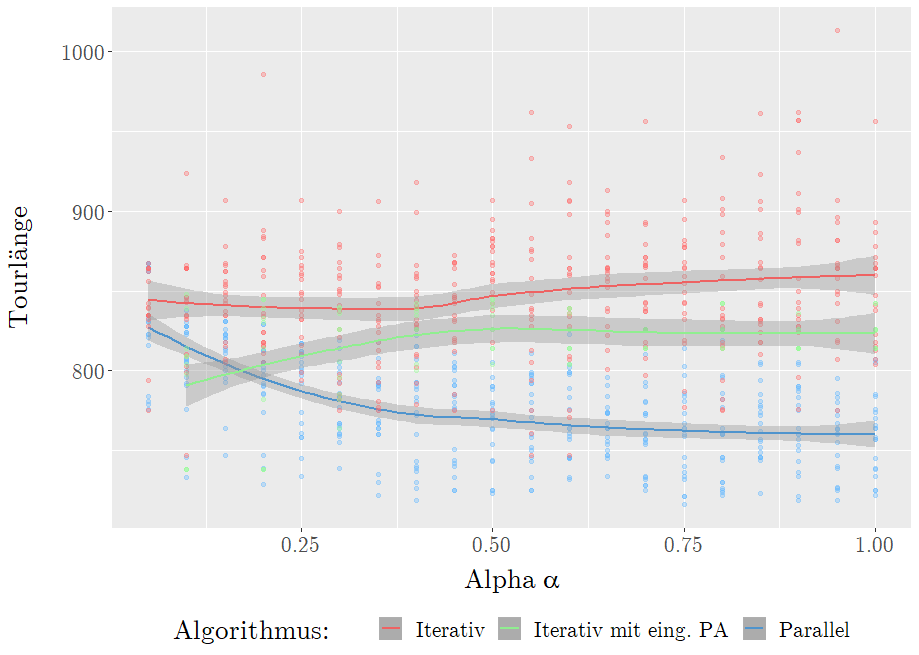
\includegraphics[width=\textwidth]{images/diagramalpha}
            \caption{Alpha $\alpha$}               
            \label{fig:iterativeAlpha}
        \end{subfigure}
        \hfill
        \begin{subfigure}[b]{0.475\textwidth}  
            \centering 
            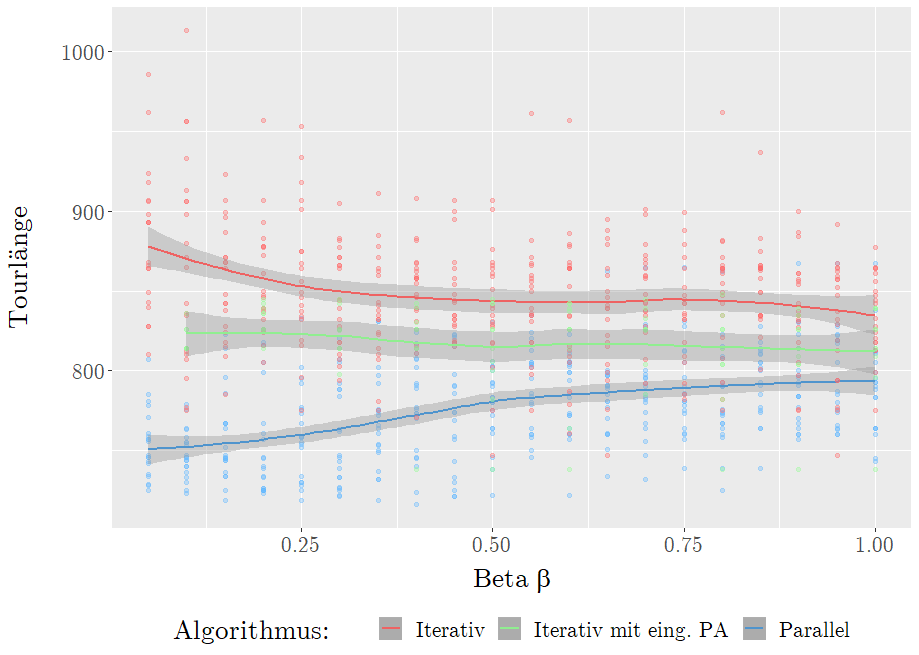
\includegraphics[width=\textwidth]{images/diagrambeta}
            \caption{Beta $\beta$}   
            \label{fig:iterativeBeta}
        \end{subfigure}
        \vskip\baselineskip
        \begin{subfigure}[b]{0.475\textwidth}   
            \centering 
            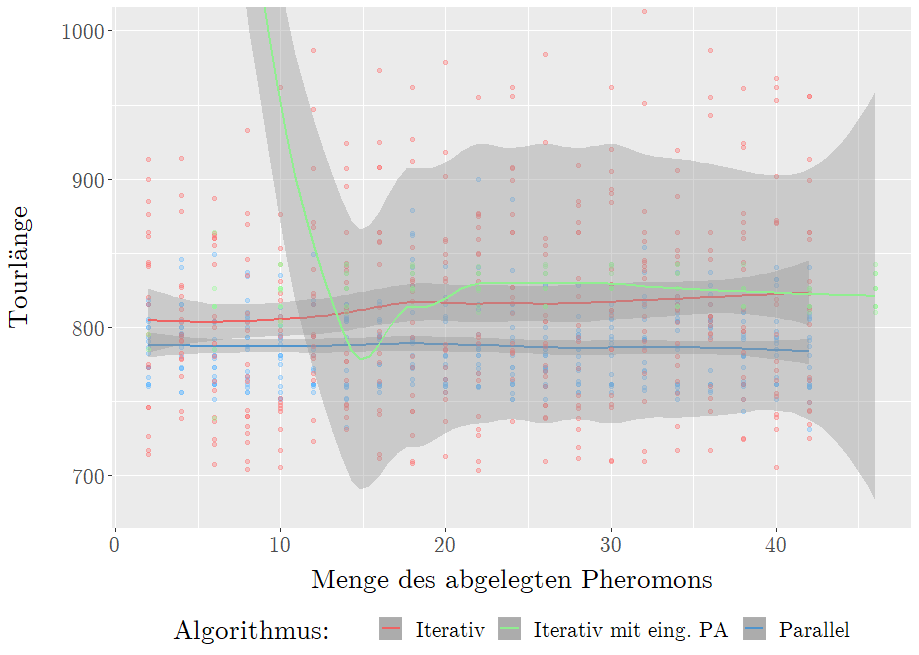
\includegraphics[width=\textwidth]{images/diagramdeposit}
            \caption{Menge des abgelegten Pheromons}   
            \label{fig:iterativeDeposit}
        \end{subfigure}
        \quad
        \begin{subfigure}[b]{0.475\textwidth}   
            \centering 
            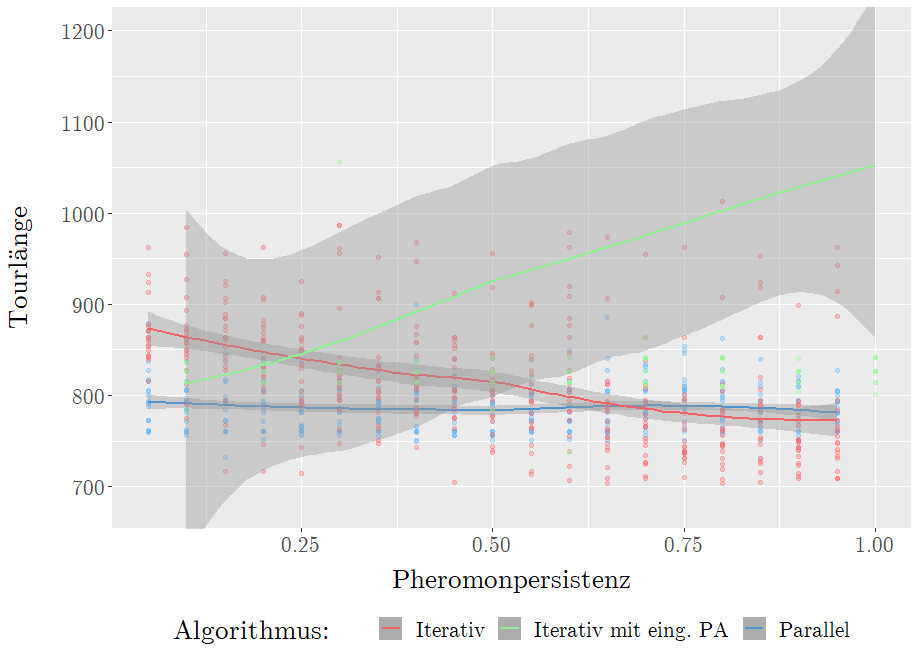
\includegraphics[width=\textwidth]{images/diagramreduction}
            \caption{Pheromonpersistenz}   
            \label{fig:iterativeReduction}
        \end{subfigure}
        \captionsetup{justification=centering}
        \caption{Abhängigkeit der Tourlänge von den einzelnen Parametern für die drei implementierten Algorithmen zur Tourkonstruktion} 
        \label{fig:ParameterDiagram}
    \end{figure}
Die in den Diagrammen dargestellten Funktionsgraphen geben den Durchschnitt der Parameterwerte an; die farbigen Punkte die jeweiligen Einzelwerte für jeden Parameter.
\\Für die Parameter Alpha $\alpha$ und Beta $\beta$ ist deutlich zu sehen, dass die beiden iterativen Algorithmen sich bei Wertänderung dieser Parameter ähnlich verhalten. Für beide Algorithmen ist die Tourlänge für einen niedrigen Wert für $\alpha$ und einen höheren Wert für $\beta$ näher am Tourlängenoptimum. Für die parallele Implementierung verhält sich dieser Sachverhalt genau umgekehrt. Die höchste Streuung der Tourlängen hat dabei der iterative Algorithmus mit einigen Ausreißern, die bis zu 50 Prozent über dem Tourlängenoptimum liegen.
\\Im Hinblick auf die Pheromonablagemenge und die Pheromonpersistenz fällt vor allem der iterative Algorithmus mit eingeschränkter Pheromonaktualisierung auf. Die beiden Parameter wirken sich enorm auf die Ergebnisse dieses Algorithmus aus. Für den Pheromonablageparameter $Q$ ergibt sich eine annäherungsweise exponentielle Funktion, die sich ungefähr bei $Q = 20$ normalisiert. Die Pheromonpersistenz $\rho$ lässt sich dagegen annäherungsweise als lineare ansteigende Funktion beschreiben. 
\\Die größte Streuung für diese Parameter im Hinblick auf die Tourlängen besitzt auch in diesem Fall der iterative Algorithmus.
\\Für die einzelnen Algorithmen sind nun die Parameterwerte in Tabelle \ref{tableParameterOptimum} für die \texttt{dantzig42}-Probleminstanz nahezu optimal:
\begin{table}[]
\centering
\resizebox{\columnwidth}{!}{%
\begin{tabular}{l|llll}
Algorithmus           & Alpha $\alpha$ & Beta $\beta$ & Pheromonablagemenge $Q$ & Pheromonpersistenz $\rho$ \\ \hline
Iterativ              & 0,1            & 1            & 10                      & 0,9                       \\
Iterativ mit eing. PA & 0,1            & 1            & 20                      & 0,1                       \\
Parallel              & 1              & 0,1          & 40                      & 0,9   \\
\multicolumn{5}{l}{}                    
\end{tabular}%
}
\captionsetup{justification=centering}
\caption[Übersicht der Parameterwerte, die bei jedem Algorithmus der Tourkonstruktion zu den besten Ergebnissen im Hinblick auf eine kurze Tourlänge führen]{Übersicht der Parameterwerte, die bei dem jeweiligen Algorithmus zu den besten Ergebnissen im Hinblick auf eine kurze Tourlänge führen}
\label{tableParameterOptimum}
\end{table}
\\Für die Auswertung der zwei implementierten Wahrscheinlichkeitsalgorithmen zeigen die Ergebnisse in Abschnitt \ref{AuswirkungWA}., dass bei Verwendung des komplexeren Wahrscheinlichkeitsalgorithmus keine besseren Ergebnisse erzielt werden, sondern lediglich die Laufzeit stark zunimmt. Dies war schon im Vorfeld zu erwarten, da der komplexe Algorithmus die Wertigkeiten der Wahrscheinlichkeiten nicht verändert, sondern die Werte nur in einen prozentualen Wert skaliert.
\\Aufgrund der ermittelten Ergebnisse ist es deswegen sinnvoller, den einfachen Wahrscheinlichkeitsalgorithmus mit einer wesentlich geringeren Berechnungszeit zu wählen.
\\Im Nachhinein wurde dennoch festgestellt, dass eine bessere Implementierung der ausführlicheren Formel (Formel \ref{eq:Prob}) zu wesentlich besseren Resultaten bei dem komplexen Wahrscheinlichkeitsalgorithmus geführt hätte.
\\\\Abschließend werden die Ergebnisse betrachtet, die bei der Anwendung aller drei Tourkonstruktionsalgorithmen auf die vier ausgewählten TSP-Probleminstanzen \texttt{burma14}, \texttt{dantzig42}, \texttt{gr120} und \texttt{si535} erreicht wurden. 
\\Während der Versuchsdurchläufe wurde festgestellt, dass bei beiden iterativen Vorgehensweisen bei Problemen mit weniger als $100$ Städten andere Parameter zu guten Ergebnissen führten als bei Problemen mit mehr als $100$ Städten. Diese unterschiedlichen Parameter finden sich zusammen mit den ausführlichen Ergebnissen in Tabelle \ref{table1} auf Seite \pageref{table1}. Die jeweils besten und schlechtesten Ergebnisse sind in Tabelle \ref{tablebestworst} zusammengefasst.
\begin{table}[]
\centering
\resizebox{\columnwidth}{!}{%
\begin{tabular}{@{}lllllll@{}}
\toprule
          &         & \multicolumn{1}{l|}{}                   & \multicolumn{2}{c|}{gefundene Routenlängen}                 & \multicolumn{2}{c}{gemessene Laufzeiten in {[}s{]}} \\
Name      & Optimum & \multicolumn{1}{l|}{}                   & Algorithmus  & \multicolumn{1}{l|}{Tourlänge $\varnothing$} & Algorithmus         & Laufzeit $\varnothing$        \\ \midrule
burma14   & 3323    & \multicolumn{1}{l|}{beste Werte}        & Parallel     & \multicolumn{1}{l|}{3323 ($0 \%$)}           & Parallel            & 0,52                          \\
          &         & \multicolumn{1}{l|}{schlechteste Werte} & Iterativ     & \multicolumn{1}{l|}{3450,2 ($3,8 \%$)}       & Iterativ ePA        & 3,31                          \\ \midrule
dantzig42 & 699     & \multicolumn{1}{l|}{beste Werte}        & Iterativ     & \multicolumn{1}{l|}{721,9 ($3,2 \%$)}        & Parallel            & 3,37                          \\
          &         & \multicolumn{1}{l|}{schlechteste Werte} & Iterativ ePA & \multicolumn{1}{l|}{824,2 ($17,9 \%$)}       & Iterativ ePA        & 23,01                         \\ \midrule
gr120     & 6942    & \multicolumn{1}{l|}{beste Werte}        & Iterativ     & \multicolumn{1}{l|}{8221,6 ($18,4 \%$)}      & Parallel            & 24,64                         \\
          &         & \multicolumn{1}{l|}{schlechteste Werte} & Iterativ ePA & \multicolumn{1}{l|}{8832 ($27,2 \%$)}        & Iterativ ePA        & 182,84                        \\ \midrule
si535     & 48450   & \multicolumn{1}{l|}{beste Werte}        & Iterativ     & \multicolumn{1}{l|}{51529,3 ($6,35 \%$)}     & Parallel            & 503,4                         \\
          &         & \multicolumn{1}{l|}{schlechteste Werte} & Parallel & \multicolumn{1}{l|}{72137,8 ($48,89 \%$)}                        & Iterativ ePA        & ($\sim$1 Stunde)              \\ \bottomrule
\multicolumn{7}{l}{}                                                                                                                                                                      
\end{tabular}%
}
\captionsetup{justification=centering}
\caption[Zusammenfassung der jeweils besten und schlechtesten Algorithmen im Bezug auf die Laufzeit und die Effektivität für jede der vier untersuchten TSP-Probleminstanzen]{Zusammenfassung der jeweils besten und schlechtesten Algorithmen im Bezug auf die Laufzeit und die Effektivität für jede der vier untersuchten TSP-Probleminstanzen. Die Prozentangabe hinter den Distanzwerten steht für die Abweichung vom Optimalwert. Die Abkürzung \glqq Iterativ ePA\grqq\, steht für den Iterativen Algorithmus mit eingeschränkter Pheromonaktualisierung.}
\label{tablebestworst}
\end{table}
\\Betrachtet man die kleinste TSP-Instanz \texttt{burma14}, so ist der parallele Tourkonstruktionsalgorithmus ideal. Dieser fand in allen Durchgängen die optimale Route. Der iterative Algorithmus erzielte die schlechtesten Ergebnisse mit einer maximalen Abweichung von $3,8 \%$. Die Laufzeit ist für alle Algorithmen bei der Anwendung auf dieses Problem akzeptabel. Die wesentlich höhere Laufzeit des iterativen Algorithmus mit eingeschränkter Pheromonaktualisierung war aufgrund des mehrfachen Durchlaufs der Tourkonstruktion zu erwarten.
\\Für die drei verbleibenden Probleme erweist sich nun der iterative Algorithmus als effektivster Algorithmus. Der iterative Algorithmus mit eingeschränkter Pheromonaktualisierung ist dagegen, sowohl was die Effektivität als auch die Laufzeit angeht, der schlechteste Algorithmus. Bei der \texttt{si535}-Probleminstanz mit $535$ Städten dauert ein Durchlauf geschätzt eine Stunde, was ihn für einen heuristischen Algorithmus bei dieser Problemgröße unbrauchbar macht. \\Die kürzesten Laufzeiten erzielt durchweg der parallele Algorithmus zur Tourkonstruktion.
\\In der nachfolgenden Abbildung \ref{img:runtimecity} ist die Laufzeit in Abhängigkeit von der Anzahl der Städte abgebildet.
\begin{figure}[!]
\captionsetup{justification=centering}
  \centering
     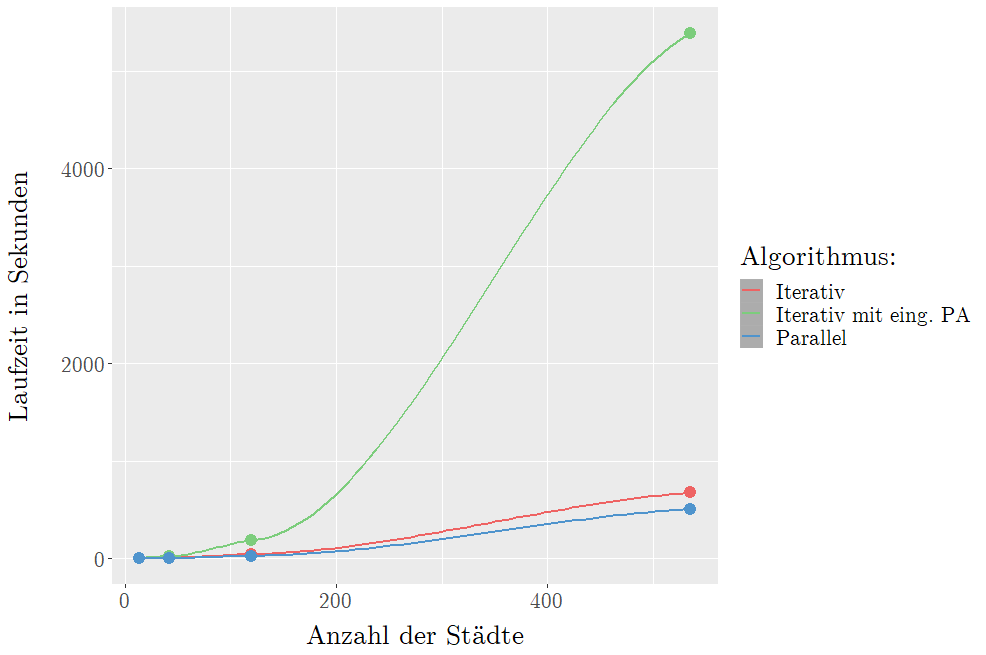
\includegraphics[width=\textwidth]{images/diagramruntimes.png}
  \caption[Darstellung der Laufzeit in Abhängigkeit von der Anzahl der Städte für alle drei implementierten Tourkonstruktionsalgorithmen]{Darstellung der Laufzeit in Abhängigkeit von der Anzahl der Städte für alle drei implementierten Tourkonstruktionsalgorithmen. Zur besseren Darstellung wurde für die y-Achse eine logarithmische Skalierung gewählt.}
  \label{img:runtimecity}
\end{figure}
\\Betrachtet man diese Graphen als eine logarithmische Funktion der Form $n log(x)$, so erhält man bei dem iterativen Algorithmus den Wert $180$ für $n$, für den iterativen Algorithmus mit eingeschränkter Pheromonaktualisierung den Wert $1439$ und für den parallelen Algorithmus den Wert $135$. Diese Werte verdeutlichen noch einmal die wesentliche höhere Laufzeit des iterativen Algorithmus mit eingeschränkter Pheromonaktualisierung im Gegensatz zu den anderen zwei Algorithmen.
\\Zusammenfassend lässt sich sagen, dass der iterative Algorithmus für mittlere und große Probleme die beste Wahl ist. Bei kleinen Problemen eignet sich der parallele Algorithmus am besten, da er dort mit hoher Wahrscheinlichkeit die optimale Lösung finden wird. Vom Gebrauch des iterativen Algorithmus mit eingeschränkter Pheromonaktualisierung ist abzuraten.
\subsection{Vergleich mit der Effektivität und Komplexität von anderen Algorithmen zur Lösung des TSP}
Verglichen mit anderen Algorithmen zur Lösung einer TSP-Instanz schneidet der ACO grade im Hinblick auf die Laufzeit eher schlecht ab. Mittlerweile gibt es eine große Zahl an exakten und heurisitischen Algorithmen, die eine wesentlich bessere Effizienz und Laufzeit besitzen. Zum Vergleich wurden zwei Implementierungen gewählt. Dies ist zum einen der \textit{Concorde TSP Solver}. Dieser stellt eine Bibliothek von Algorithmen zur Lösung des TSP und anderen Netzwerkoptimierungsproblemen bereit. Dabei baut er auf \textit{CPLEX} auf, einem Programmsystem zur Lösung von Optimierungsproblemen mithilfe der mathematischen Optimierung. Das Projekt wurde in der Programmiersprache C geschrieben. Mithilfe dieses Lösungsverfahrens wurden bis auf vier Instanzen alle Probleme der TSPLIB gelöst \cite{Concorde}.
\\Zum anderen wird der heuristische Lin-Kernighan-Algorithmus herangezogen, der 1973 von Brian W. Kernighan und Shen Lin veröffentlicht wurde \cite{TSP}.
\\Tabelle \ref{tableextern} zeigt die erzielten Laufzeiten und Tourlängen der zwei externen Algorithmen und des eigenen ACO.
\begin{table}[!]
\centering
\resizebox{\columnwidth}{!}{%
\begin{tabular}{@{}llllll@{}}
\toprule
          &         &                                & \multicolumn{3}{c}{Algorithmus}         \\
Name      & Optimum & \multicolumn{1}{l|}{}          & Concorde CPLEX & Lin-Kernighan & ACO    \\ \midrule
burma14   & 3323    & \multicolumn{1}{l|}{Tourlänge} & 3323           & 3323          & 3323   \\
          &         & \multicolumn{1}{l|}{Laufzeit in s}  & 0,1            & 0,05          & 0,52   \\ \midrule
dantzig42 & 699     & \multicolumn{1}{l|}{Tourlänge} & 699            & 699           & 722    \\
          &         & \multicolumn{1}{l|}{Laufzeit in s}  & 0,4            & 0,1           & 4,41   \\ \midrule
gr120     & 6942    & \multicolumn{1}{l|}{Tourlänge} & 6942           & 6942          & 8222   \\
          &         & \multicolumn{1}{l|}{Laufzeit in s}  & 2,2            & 0,7           & 42,77  \\ \midrule
si535     & 48450   & \multicolumn{1}{l|}{Tourlänge} & 48450          & 48574         & 51529  \\
          &         & \multicolumn{1}{l|}{Laufzeit in s}  & 30,1           & 4,1           & 673,59 \\ \bottomrule
          &         &                                &                &               &       
\end{tabular}%
}
\caption{Übersicht über die gefundenen Routenlängen und Laufzeiten der vier in dieser Arbeit untersuchten TSP-Instanzen im Vergleich mit dem Concorde TSP Solver und der Lin-Kernighan-Heurisitik}
\label{tableextern}
\end{table}
\\Es zeigt sich deutlich, dass der implementierte ACO für die Lösung einer TSP-Instanz nicht die beste Wahl ist. Dies war schon von Beginn an zu erwarten, da der Ameisenalgorithmus ein evolutionärer Algorithmus ist, der als Metaheuristik eine andere Vorgehensweise zur Lösung einer TSP-Instanz benutzt. Die Eigenschaft, eine Metaheuristik zu sein, ermöglicht diesem Algorithmus aber eine Anwendung auf ein breites Spektrum anderer Optimierungsprobleme. 
\newpage
\section{Zusammenfassung und Ausblick}
Die in dieser Arbeit vorgestellten Implementierungen des Ameisenalgorithmus sind eine durchaus nutzbare Möglichkeit zur Lösung des Travelling Salesman Problems. Im Vergleich zu exakten Lösungsalgorithmen erzielen sie zwar meistens keine optimalen Tourlängen, liefern aber als heuristischer Ansatz vertretbare Resultate.
\\Es hat sich gezeigt, dass der parallele Algorithmus zur Tourkonstruktion bei kleinen TSP-Instanzen gute und sogar optimale Resultate erreicht, während der iterative Algorithmus zur Tourkonstruktion für größere Probleme die besten Ergebnisse erzielt. Der iterative Algorithmus mit eingeschränkter Pheromonaktualisierung ist jedoch im Hinblick sowohl auf die Laufzeit als auch auf die Effizienz eine ungünstige Wahl. Für optimale Ergebnisse ist hier eine sehr hohe Zahl an Iterationen notwendig, da die Pheromonspuren pro Iteration nur minimal aktualisiert werden.
\\Der implementierte einfache Wahrscheinlichkeitsalgorithmus zur Ermittlung der jeweils nächsten Stadt während der Tourkonstruktion hilft dabei, wertvolle Laufzeit bei unveränderten Ergebnissen einzusparen. 
\\Insgesamt kann die Laufzeit der Implementierungen durch die Nutzung von Multithreading verbessert werden.
\\Außerdem wurden die Auswirkungen der einzelnen Parameter ausgiebig untersucht und dabei festgestellt, dass für unterschiedliche Problemgrößen unterschiedliche Parameterwerte bessere Ergebnisse liefern.
Dies lässt erkennen, dass eine dynamische Skalierung der Parameter für eine optimale Lösung zwingend erforderlich ist; eine weitere Untersuchung dieser Tatsache bietet sich deshalb als Thema für zukünftige Projekte an.
\\Der Ameisenalgorithmus und sein Einsatz als Lösungsverfahren für kombinatorische Optimierungsprobleme ist ein wichtiger Baustein in der Erforschung von evolutionären Algorithmen. Er ist somit auch eng mit dem informatischen Teilgebiet der Künstlichen Intelligenz verknüpft. Das Verständnis über die Funktionsweise dieses Algorithmus dient deswegen auch zukunftsweisend als eine Grundlage zur Entwicklung von Projekten in diesem Bereich.
\newpage
\appendix
\section{Erklärung der implementierten grafischen Oberfläche}
\begin{figure}
\captionsetup{justification=centering}
  \centering
     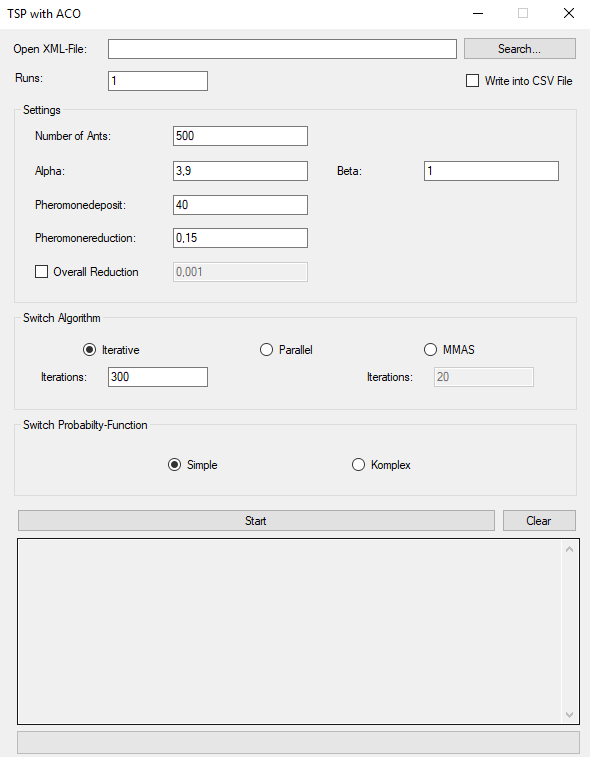
\includegraphics[width=0.7\textwidth]{images/TSPACOGUI.png}
  \caption[Grafische Oberfläche der Implementierung des Ameisenalgorithmus in C\texttt{++}]{Grafische Oberfläche des Programms}
  \label{img:gui}
\end{figure}
Der Button \textbf{Search...} öffnet einen neuen Filedialog, mit dem die gewünschte Probleminstanz im XML-Format geladen werden kann. Alternativ kann der Dateipfad auch in das nebenstehende Textfeld eingegeben werden.
\\\\Der Paramater im Textfeld \textbf{Runs} gibt an, wie oft das gesamte Programm ausgeführt werden soll. Dies ist hilfreich bei der Ermittlung von Durchschnittswerten für einzelne festgelegte Parameter.
\\\\Unter \textbf{Settings} befinden sich alle konfigurierbaren Parameter, die Einfluss auf den Algorithmus haben. 
\\\textbf{Number of Ants} gibt die Anzahl der Ameisen an, welche die Route konstruieren. \textbf{Alpha} steht für die Wichtigkeit der Pheromonspur, \textbf{Beta} für die Wichtigkeit der Distanz bei der Ermittlung der nächsten Stadt im Verlauf der Tourkonstruktion. Der Parameter \textbf{Pheromondeposit} gibt die Menge des ablegten Pheromons an, während \textbf{Pheromonereduction} für die Verdunstungsmenge steht.
\\\\Unter \textbf{Switch Algorithm} kann der gewünschte Algorithmus zur Berechnung der kürzesten Route gewählt werden. \textbf{Iterations} gibt dabei für den iterativen Algorithmus die Anzahl von Iterationen an, nach denen der Algorithmus abbricht, wenn keine kürzere Route gefunden wurde. Analag gibt er für die Option \textbf{Iterative with restricted Pheromoneupdate} an, wie oft alle Ameisen ihre Tour konstruieren.
\\\\Mit \textbf{Switch Probability-Function} kann zwischen einem einfachen und einem komplexeren Algorithmus zur Ermittlung der nächsten jeweiligen Stadt bei der Erstellung der Route ausgewählt werden.
\\\\Ein Klick auf den Button \textbf{Start} startet den Algorithmus. Die Ausgabe erfolgt in das untenstehende Textfeld, welches mit dem Button \textbf{Clear} geleert werden kann.
\\\\Möchte man zudem eine Ausgabe in eine Tabellendatei erhalten, muss oben rechts die Funktion \textbf{Write into CSV File} aktiviert werden.
\newpage
\section{Hinweise zur Nutzung des Programms als Konsolenapplikation}
Die Implementierung des Ameisenalgorithmus zur Lösung von TSP-Probleminstanzen kann auch auf Konsolenbasis unter Windows genutzt werden. Hierbei werden der Pfad und die einzelnen Optionen als Runtime-Parameter übergeben. Insgesamt müssen dabei jeweils 13 Parameter gesetzt werden.
\begin{enumerate}
\item Dateipfad (Datei muss dabei als \texttt{XML}-Datei vorliegen)
\item Anzahl der Ameisen, die eine Tour generieren
\item Gewünschter Algorithmus: \glqq 0\grqq\, entspricht dem iterativen Algorithmus, \glqq 1\grqq\, dem parallelen Algorithmus und \glqq 2\grqq\, dem iterativen Algorithmus mit eingeschränkter Pheromonaktualisierung
\item Wert für die Menge an abgelegtem Pheromon $Q$ - sollte zwischen $0.05$ und $80$ liegen
\item Wert für die Pheromonverdunstung $1 - \rho$ - sollte zwischen $0.01$ und $0.99$ liegen
\item Wert für den Parameter Alpha $\alpha$ - sollte zwischen $0.01$ und $1$ liegen
\item Wert für den Parameter Beta $\beta$ - sollte zwischen $0.01$ und $1$ liegen
\item Schalter für eine optionale allgemeine Reduzierung der Pheromonmatrix nach jeder Tourkonstruktion - für \glqq 0\grqq\, ist die Option deaktiviert, für \glqq 1\grqq\, aktiviert
\item Wert für die optionale allgemeine Reduzierung der Pheromonmatrix - sollte zwischen $0.001$ und $0.1$ liegen
\item Anzahl der Iterationen für den Iterativen Algorithmus, bei der Wahl von anderen Algorithmen \glqq 0\grqq\, eintragen
\item Anzahl der Iterationen beim Iterativen Algorithmus mit eingeschränkter Pheromonaktualisierung, bei der Wahl von anderen Algorithmen \glqq 0\grqq\, eintragen
\item Schalter für den Wahrscheinlichkeitsalgorithmus - bei \glqq 0\grqq\, wird der einfache Algorithmus verwendet, bei \glqq 1\grqq\, der komplexe Algorithmus
\item Schalter für die Ausgabe in eine CSV-Datei - für \glqq 0\grqq\, ist die Option deaktiviert, für \glqq 1\grqq\, aktiviert
\end{enumerate}
Für die Verwendung des Iterativen Algorithmus mit $1000$ Ameisen und einer Iterationsschwelle von $500$ zur Lösung der \texttt{burma14}-Probleminstanz könnte der Prozessaufruf so aussehen:
\lstset { %
    language=C++,
    backgroundcolor=\color{black!5}, % set backgroundcolor
    basicstyle=\footnotesize,% basic font setting
    numbers=none
}
\begin{lstlisting}
TSPACO.exe burma14.xml 1000 1 40.0 0.14 1.0 0.25 0 0.001 500 0 0 0
\end{lstlisting}
\newpage
\section{Erklärung der Dateien auf dem beigefügten Datenträger}
Der beigefügte Datenträger enthält vier Ordner, in dem sich alle wichtigen Dateien befinden, die im Rahmen dieser Arbeit erstellt oder benötigt wurden.
\\\\In dem Ordner \textbf{Artikel} befinden sich wissenschaftliche Artikel und Paper, die als Quellen bei der Erstellung dieser Arbeit benutzt wurden. 
\\Der Ordner \textbf{Executables} enthält zwei auf Windows ausführbare Dateien, welche die Implementierung des Ameisenalgorithmus in C\texttt{++} darstellen. Zum einen ist das die in Anhang A vorgestellte grafische Oberfläche, zum anderen die in Anhang B erklärte Konsolenapplikation.
\\Den Programmcode des Projektes findet man im Ordner \textbf{Sourcecode}, sowohl für die GUI als auch für die konsolenbasierte Anwendung.
\\Für ein einfacheres Testen beider Programme befinden sich im Ordner \textbf{TSPLIB-Instanzen} die auch in dieser Arbeit untersuchten TSPLIB-Probleminstanzen.
\\Letztendlich ist die Bachelorarbeit als PDF im Hauptverzeichnis des Datenträgers abgelegt.
\\\\Alle beigefügten Dateien befinden sich außerdem als Repository auf Github und können unter folgendem Link eingesehen bzw. geklont werden:
\\\\\texttt{https://github.com/Samykolon/TSPACO}
\newpage
\section{Abbildungs-, Tabellen- und Algorithmenverzeichnis}
\listoffigures
\listoftables
\newpage
\listof{algorithm}{Algorithmenverzeichnis}
\newpage
\bibliography{literatur}{}
\addcontentsline{toc}{section}{Literatur} 
\end{document}